\documentclass[11pt]{article}
% ---------- Preamble: shared setup, diagram and evidence macros ----------
% Policy: all body text, headings, captions, tables and callouts are BLACK.
% Colour appears ONLY inside TikZ diagrams.
\usepackage[T1]{fontenc}
\usepackage[utf8]{inputenc}
\usepackage[a4paper,margin=1in]{geometry}
\usepackage{graphicx}
\usepackage{xcolor}
\usepackage{booktabs}
\usepackage{colortbl}
\usepackage{array}
\usepackage{tabularx}
\usepackage{enumitem}
\usepackage{longtable}
\usepackage{float}
\usepackage{caption}
\usepackage{amssymb}
\usepackage{fancyhdr}
\usepackage{titlesec}
\usepackage{listings}
\usepackage{tikz}
\usetikzlibrary{positioning,arrows.meta,calc,fit,backgrounds,shapes.geometric}
\usepackage[hidelinks]{hyperref}

% ---------- Diagram-only palette (never used for text) ----------
\definecolor{accent}{HTML}{2C6E91}
\definecolor{accentlt}{HTML}{E6EEF3}
\definecolor{good}{HTML}{2E7D4F}
\definecolor{goodlt}{HTML}{E4F1E9}
\definecolor{bad}{HTML}{B23A3A}
\definecolor{badlt}{HTML}{F6E5E4}
\definecolor{net1}{HTML}{E7F0F7}
\definecolor{net2}{HTML}{FBEFE3}
\definecolor{net3}{HTML}{EAF2EA}
\definecolor{dslate}{HTML}{45566B}
% grayscale tones for placeholders and code frames (neutral, not colour)
\definecolor{boxframe}{gray}{0.0}
\definecolor{boxfill}{gray}{0.96}
\definecolor{boxtext}{gray}{0.25}
\definecolor{coderule}{gray}{0.55}

% ---------- Section styling: black ----------
\titleformat{\section}{\color{black}\Large\bfseries}{\thesection}{0.6em}{}
\titleformat{\subsection}{\color{black}\large\bfseries}{\thesubsection}{0.6em}{}
\titleformat{\subsubsection}{\color{black}\normalsize\bfseries}{\thesubsubsection}{0.6em}{}
\titlespacing*{\section}{0pt}{1.4em}{0.7em}

% ---------- Header / footer: black ----------
\pagestyle{fancy}
\fancyhf{}
\renewcommand{\headrulewidth}{0.4pt}
\renewcommand{\footrulewidth}{0pt}
\fancyhead[L]{\small CS6008 Network Security}
\fancyhead[R]{\small Assignment 2: DNS Security}
\fancyfoot[C]{\small\thepage}

% ---------- Listings: black text, white ground, plain frame ----------
\lstdefinestyle{term}{
  basicstyle=\ttfamily\footnotesize\color{black},
  backgroundcolor=\color{white},
  breaklines=true,
  breakatwhitespace=false,
  columns=fullflexible,
  keepspaces=true,
  frame=single,
  rulecolor=\color{coderule},
  framesep=6pt,
  xleftmargin=10pt,
  xrightmargin=4pt,
  aboveskip=10pt,
  belowskip=8pt,
  showstringspaces=false
}
\lstset{style=term}

% ---------- Evidence figures ----------
% Each figure embeds its screenshot AUTOMATICALLY, found by the figure's label:
% a figure with \label{fig:p2-attack} looks for an image called p2-attack.
% It searches, in order:  images/p2-attack.png, images/p2-attack.PNG,
% images/p2-attack.jpg, images/p2-attack.jpeg, images/p2-attack.pdf, and the
% same five names at the project root.  As soon as one of those files exists
% the picture appears; until then a gray "reserved space" box is shown that
% prints the exact filename it is waiting for.  So the ONLY thing you have to do
% is name each screenshot after its figure (see the list in SCREENSHOTS.md) and
% drop them in an images/ folder.  Nothing in report.tex needs editing.
\graphicspath{{images/}{./}}

% strip the leading "fig:" from a label so we can build the image filename
\def\stripfigcolon fig:#1\stripfigend{#1}
\newcommand{\figimgname}[1]{\expandafter\stripfigcolon#1\stripfigend}

% try to include <base> with any known folder+extension; run #2 if none found
\newcommand{\tryshot}[2]{% #1 = basename (e.g. p2-attack), #2 = fallback code
  \IfFileExists{images/#1.png}{\includegraphics[width=0.92\linewidth]{images/#1.png}}{%
  \IfFileExists{images/#1.PNG}{\includegraphics[width=0.92\linewidth]{images/#1.PNG}}{%
  \IfFileExists{images/#1.jpg}{\includegraphics[width=0.92\linewidth]{images/#1.jpg}}{%
  \IfFileExists{images/#1.jpeg}{\includegraphics[width=0.92\linewidth]{images/#1.jpeg}}{%
  \IfFileExists{images/#1.pdf}{\includegraphics[width=0.92\linewidth]{images/#1.pdf}}{%
  \IfFileExists{#1.png}{\includegraphics[width=0.92\linewidth]{#1.png}}{%
  \IfFileExists{#1.jpg}{\includegraphics[width=0.92\linewidth]{#1.jpg}}{%
  #2}}}}}}}%
}

% #1 = caption, #2 = what the screenshot should show, #3 = suggested file,
% #4 = label. #5 = minipage height for the fallback box.
\newcommand{\shotboxinner}[5]{%
\begin{figure}[H]
\centering
\edef\figbase{\figimgname{#4}}%
\tryshot{\figbase}{%
  \setlength{\fboxsep}{0pt}%
  \fcolorbox{boxframe}{boxfill}{%
  \begin{minipage}[c][#5][c]{0.90\linewidth}
  \centering
  {\small\itshape\color{boxtext} Space reserved for screenshot}\\[3pt]
  {\small\color{boxtext} #2}\\[5pt]
  {\footnotesize\color{boxtext} Save screenshot as \texttt{images/\figbase.png} \quad (source: \texttt{#3})}
  \end{minipage}}%
}%
\caption{#1}
\label{#4}
\end{figure}}

\newcommand{\shot}[4]{\shotboxinner{#1}{#2}{#3}{#4}{40mm}}
\newcommand{\shottall}[4]{\shotboxinner{#1}{#2}{#3}{#4}{58mm}}

% ---------- Callout: black framed box ----------
\newcommand{\takeaway}[1]{%
\par\smallskip\noindent
\setlength{\fboxsep}{7pt}%
\fbox{\parbox{\dimexpr\linewidth-2\fboxsep-2\fboxrule\relax}{\small #1}}%
\par\smallskip}

\newcolumntype{Y}{>{\raggedright\arraybackslash}X}
\captionsetup{font=small,labelfont=bf,textfont=normal}

\begin{document}

% =====================================================================
% TITLE
% =====================================================================
\begin{titlepage}
    \centering

    \vspace*{0.6cm}

    % --- Institute logo ---
    % Put your logo at images/iitb_logo.png (or iitb_logo.png next to this file).
    % If it is not present the title page still compiles, just without the logo.
    \IfFileExists{images/iitb_logo.png}{\includegraphics[width=6.2cm]{images/iitb_logo.png}}{%
      \IfFileExists{iitb_logo.png}{\includegraphics[width=6.2cm]{iitb_logo.png}}{}}

    \vspace{0.8cm}

    {\Large\bfseries Indian Institute of Technology Bombay\par}

    \vspace{0.25cm}

    {\large Department of Computer Science and Engineering\par}

    \vspace{0.35cm}

    {\large\bfseries CS6008 : Network Security\par}

    \vspace{1.4cm}

    \rule{0.7\linewidth}{0.6pt}

    \vspace{0.6cm}

    {\LARGE\bfseries DNS Security: Building, Attacking, and Defending a Hierarchical DNS\par}

    \vspace{0.35cm}

    {\Large Assignment Report\par}

    \vspace{0.6cm}

    \rule{0.7\linewidth}{0.6pt}

    \vspace{1.6cm}

    \begin{tabular}{rl}
        \textbf{Name}     & Reman Krishnan, Anant Kashid\\[4pt]
        \textbf{Roll No.} & 26D0365, 26V0011 \\[4pt]
        \textbf{Course}   & CS6008: Network Security \\[4pt]
        \textbf{Programme}& Ph.D / B.Tech
    \end{tabular}

    \vfill

    \vspace{1.0cm}

    {\large September 2026\par}

\end{titlepage}

\newpage
\tableofcontents
\newpage

\clearpage

% =====================================================================
% OVERVIEW
% =====================================================================
\section{Overview and Methodology}

DNS answers, in their original and still most common form, travel as
unauthenticated cleartext. Anyone who sits on the path between a client and the
nameservers it depends on can read a query as it passes and, just as easily,
forge the reply that comes back. This single property, the absence of any proof
that an answer came from the party entitled to give it, is the thread that runs
through the whole assignment. Each phase of this report either exploits that
property from a particular position or adds a mechanism intended to remove it at
a particular layer.

The methodology is deliberately uniform across the seven phases, so that the
results can be compared like for like. Every phase begins by deploying or
extending the containerised hierarchy, then verifies that the deployment behaves
as intended with the attacker absent or passive, and finally mounts the attack
and records exactly what the resolver cached, what the client received, and what
the packet capture showed. Keeping the structure constant means that any change
in outcome from one phase to the next can be attributed to the one thing that
changed between them, which is usually a single defensive mechanism or a single
configuration choice. The attacker itself is kept as constant as possible and is
simply relocated or extended, rather than rewritten, so that a defence is tested
against the same adversary that defeated the layer before it.

A short note on terminology is useful before the details begin. The resolver is
the recursive, caching server that the client asks. The authoritative servers are
the root, the \texttt{com} top-level domain, and the \texttt{example.com} domain
servers that actually hold the data. The attacker is a single container that is
placed on whichever subnet the phase in question requires. All addresses are fixed
in advance and are reused unchanged in every phase, which is what makes the captures
directly comparable.

\subsection{Environment and tooling}

Every node in the laboratory is a Docker container with a fixed address on one of
three isolated bridge networks. Isolation is a property of the topology rather
than of any firewall rule. No subnet has a direct link to any other, so every
packet that crosses from one subnet to another must pass through one of two
routers, and those routers are the only containers permitted to forward traffic.
This matters for the attacks that follow, because the adversary never has to
defeat a filter. It only has to occupy a position that the topology already
forces traffic through.

\begin{table}[H]
\centering
\small
\begin{tabularx}{\linewidth}{l l l Y}
\toprule
\textbf{Component} & \textbf{Subnet} & \textbf{Address} & \textbf{Role} \\
\midrule
client      & client        & 172.16.1.10  & End host issuing lookups and web requests \\
webserver   & client        & 172.16.1.20  & Serves the legitimate \texttt{example.com} site over HTTP \\
rogue-web   & client        & 172.16.1.30  & Adversary's web server hosting the defacement page \\
resolver    & resolver      & 172.16.2.10  & Recursive caching resolver that validates DNSSEC from Phase 3 \\
root-ns     & authoritative & 172.16.3.10  & Authoritative server for the root zone (\texttt{.}) \\
tld-ns      & authoritative & 172.16.3.20  & Authoritative server for the \texttt{.com} zone \\
domain-ns   & authoritative & 172.16.3.30  & Authoritative server for \texttt{example.com} \\
edge-router & client/resolver & 172.16.1.2 / 172.16.2.2 & Routes client to resolver traffic, no NAT \\
core-router & resolver/auth   & 172.16.2.3 / 172.16.3.3 & Routes resolver to authoritative traffic, no NAT \\
attacker    & resolver (P2--5) & 172.16.2.100 & On-path adversary on the resolver subnet \\
attacker    & client (P6--7)   & 172.16.1.100 & The same adversary, moved to the client's last mile \\
\bottomrule
\end{tabularx}
\caption{Fixed assignment of containers to subnets and addresses, used unchanged across all phases.}
\label{tab:components}
\end{table}

The DNS daemon on every nameserver and on the resolver is BIND, confirmed at
version 9.20.x on each node. The evidence for Phases 1 to 4 was captured with the
package 9.20.30, and a few of the later phases with 9.20.23 from Debian
backports, a difference that reflects only when those container images happened
to be rebuilt. Both are BIND 9.20.x, and the point-release gap does not affect any
behaviour observed in this report. Inspection of results uses \texttt{dig},
\texttt{delv}, \texttt{kdig}, and \texttt{curl}, with \texttt{tcpdump} and
\texttt{tshark} for packet capture. The private certificate authority and the
resolver's TLS certificate are produced with OpenSSL. Routing is plain Linux IP
forwarding through \texttt{iproute2}, with static routes on every node and no
network address translation anywhere, so that addresses stay honest from end to
end and a capture shows the real source and destination of every packet.

A constraint worth stating at the outset is that every attack program was written
in C using \texttt{libpcap}, which both captures packets off the wire and injects
crafted ones back onto it through \texttt{pcap\_sendpacket}. High-level spoofing
or DNS frameworks were not used for the attacks. This keeps the adversary honest
about what an on-path attacker actually has to do, namely parse raw frames,
rewrite only the fields it cares about, recompute the IP and UDP checksums, and
inject the result, rather than hiding that machinery behind a library call. The
inspection tools named above are used only to verify results.

\subsection{Privilege model}

The privilege policy follows the principle of least authority and underpins the
isolation claim. The two routers carry \texttt{NET\_ADMIN} and are the only nodes
with IP forwarding enabled. They hold the routing table entries that join the
subnets and, from Phase 2 onward, the diversion routes that steer traffic through
the attacker. Every other node receives \texttt{NET\_ADMIN} only so that it can
install the static routes it needs to reach off-subnet addresses through its local
router, and none of them forward, bridge, or translate. The attacker additionally
holds \texttt{NET\_RAW}, which is what \texttt{libpcap} requires to capture and
inject at the link layer. Nothing in the laboratory is granted more capability
than its role demands.

\subsection{The laboratory topology}

Figure~\ref{fig:topology} shows the full deployment. The three coloured regions
are the three bridge networks. The routers straddle two networks each and are
drawn on the boundary between them, which is exactly where they sit in the address
plan. The attacker is shown in both of its positions, on the resolver subnet for
Phases 2 to 5 and on the client subnet for Phases 6 and 7, because the same
adversary is simply relocated as the defences push the interesting attack surface
closer to the client.

\begin{figure}[H]
\centering
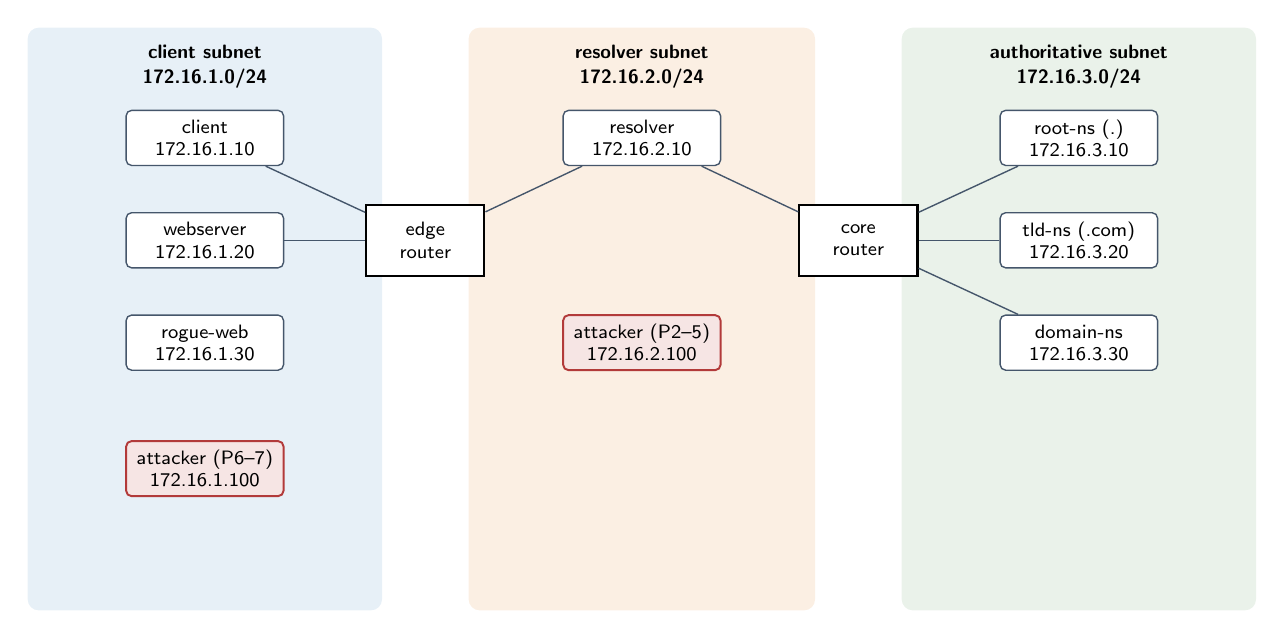
\begin{tikzpicture}[
  font=\sffamily\scriptsize,
  box/.style={draw=dslate,rounded corners=2pt,fill=white,minimum width=20mm,minimum height=7mm,align=center,line width=0.5pt},
  rtr/.style={draw=black,fill=white,minimum width=15mm,minimum height=9mm,align=center,line width=0.8pt},
  atk/.style={draw=bad,fill=badlt,rounded corners=2pt,minimum width=20mm,minimum height=7mm,align=center,line width=0.7pt},
  lbl/.style={font=\sffamily\bfseries\scriptsize}
]
\begin{scope}[on background layer]
  \fill[net1,rounded corners=4pt] (-0.6,-5.4) rectangle (3.9,2.0);
  \fill[net2,rounded corners=4pt] (5.0,-5.4) rectangle (9.4,2.0);
  \fill[net3,rounded corners=4pt] (10.5,-5.4) rectangle (15.0,2.0);
\end{scope}
\node[lbl] at (1.65,1.7) {client subnet};
\node[lbl] at (1.65,1.35) {172.16.1.0/24};
\node[lbl] at (7.2,1.7) {resolver subnet};
\node[lbl] at (7.2,1.35) {172.16.2.0/24};
\node[lbl] at (12.75,1.7) {authoritative subnet};
\node[lbl] at (12.75,1.35) {172.16.3.0/24};
\node[box] (client) at (1.65,0.6) {client\\172.16.1.10};
\node[box] (web) at (1.65,-0.7) {webserver\\172.16.1.20};
\node[box] (rogue) at (1.65,-2.0) {rogue-web\\172.16.1.30};
\node[atk] (atkc) at (1.65,-3.6) {attacker (P6--7)\\172.16.1.100};
\node[box] (res) at (7.2,0.6) {resolver\\172.16.2.10};
\node[atk] (atkr) at (7.2,-2.0) {attacker (P2--5)\\172.16.2.100};
\node[box] (root) at (12.75,0.6) {root-ns (.)\\172.16.3.10};
\node[box] (tld) at (12.75,-0.7) {tld-ns (.com)\\172.16.3.20};
\node[box] (dom) at (12.75,-2.0) {domain-ns\\172.16.3.30};
\node[rtr] (edge) at (4.45,-0.7) {edge\\router};
\node[rtr] (core) at (9.95,-0.7) {core\\router};
\draw[dslate,line width=0.5pt] (client) -- (edge);
\draw[dslate,line width=0.5pt] (res) -- (edge);
\draw[dslate,line width=0.5pt] (res) -- (core);
\draw[dslate,line width=0.5pt] (root) -- (core);
\draw[dslate,line width=0.5pt] (tld) -- (core);
\draw[dslate,line width=0.5pt] (dom) -- (core);
\draw[dslate,line width=0.5pt] (web) -- (edge);
\end{tikzpicture}
\caption{The laboratory topology. Three isolated bridge networks are joined only by two forwarding routers. The adversary is the same container in two positions, on the resolver subnet for Phases 2 to 5 and relocated to the client's last mile for Phases 6 and 7.}
\label{fig:topology}
\end{figure}

A note on reproducibility applies to the whole submission. Each phase directory
contains its own Compose file, zone and daemon configuration, router and diversion
scripts, attack source with a build command, and a README listing the exact
commands to deploy, attack, and verify. A grader on a clean checkout, with only
the host tools listed above, can reproduce the results from that README alone,
because the attack programs discover the resolver's hardware address and the
relevant interface at run time rather than hard-coding them. Compiled binaries,
signed zones, generated keys, and built images are regenerated from source and are
kept out of the committed tree.

\clearpage

% =====================================================================
% PHASE 1
% =====================================================================
\section{Building the DNS Hierarchy (Phase 1)}

\subsection{Objective}

The first phase has no attacker. Its purpose is to build the baseline that every
later phase extends and to prove two things about it. The first is that it resolves
names correctly through a genuine iterative lookup. The second is that its subnets
are isolated, so that the only way between them is through a router. Getting this
right is what makes the later attacks meaningful, because an attack is only
interesting if the thing it breaks was working properly to begin with.

\subsection{Design and implementation}

The hierarchy is the textbook three tiers. The root nameserver delegates
\texttt{com.} to the TLD server, the TLD server delegates \texttt{example.com.} to
the domain server, and the domain server holds the A records for
\texttt{example.com} and \texttt{www.example.com}, both pointing at the web server
at 172.16.1.20. The resolver is recursive, and in this phase DNSSEC validation is
deliberately left off, because the whole point of Phase 1 is to establish the
unprotected baseline. The zone file for \texttt{example.com} is small and
readable.

\begin{lstlisting}[language=,caption={The example.com zone served by domain-ns in Phase 1 (zones/db.example.com).}]
$ORIGIN example.com.
$TTL 300
@   IN SOA ns.example.com. hostmaster.example.com. (
        2026102201 3600 600 86400 300 )
@   IN NS  ns.example.com.
ns  IN A   172.16.3.30
@   IN A   172.16.1.20
www IN A   172.16.1.20
\end{lstlisting}

Reachability is arranged entirely with static routes and IP forwarding, and no
NAT is used anywhere, so that the addresses a capture shows are the real ones.
Table~\ref{tab:p1-routes} lists the route that each node actually carries, taken
from the deployment. The pattern is simple to state. Every non-router node has a
connected route for its own subnet and one static route for each off-subnet
destination it needs, pointed at the router on its segment, while the two routers
have only their two connected subnets and are the sole nodes with forwarding
enabled.

\begin{table}[H]
\centering
\small
\begin{tabularx}{\linewidth}{l Y l}
\toprule
\textbf{Node} & \textbf{Static route(s) installed} & \textbf{IP forwarding} \\
\midrule
client      & 172.16.2.0/24 via 172.16.1.2 (edge) & off \\
resolver    & 172.16.1.0/24 via 172.16.2.2 (edge), and 172.16.3.0/24 via 172.16.2.3 (core) & off \\
root-ns     & 172.16.2.0/24 via 172.16.3.3 (core) & off \\
tld-ns      & 172.16.2.0/24 via 172.16.3.3 (core) & off \\
domain-ns   & 172.16.2.0/24 via 172.16.3.3 (core) & off \\
edge-router & connected to 172.16.1.0/24 and 172.16.2.0/24 & \textbf{on} \\
core-router & connected to 172.16.2.0/24 and 172.16.3.0/24 & \textbf{on} \\
\bottomrule
\end{tabularx}
\caption{Static routes and forwarding state per node, from the deployed hierarchy. Only the two routers forward, which is what makes the subnets reachable only through them.}
\label{tab:p1-routes}
\end{table}

The client is configured to use the resolver as its only nameserver, through a
\texttt{resolv.conf} that names 172.16.2.10 with a short timeout, so that every
lookup the client makes is a recursive query to the resolver rather than a direct
query to any authoritative server. The root hints and the glue records name the
nameservers at their true 172.16.3.x addresses, so the resolver performs a genuine
iterative walk.

\subsection{Verification}

Three checks establish that the baseline works. First, the BIND version is
confirmed on each server, so that later behaviour can be attributed to
configuration rather than to a version quirk.

\begin{lstlisting}[language=,caption={BIND version confirmed on every server (evidence/bind-versions.txt).}]
--- resolver / root-ns / tld-ns / domain-ns ---
BIND 9.20.30-1~deb13u1-Debian (Stable Release)
\end{lstlisting}

Second, from the client, \texttt{dig example.com} returns 172.16.1.20 and
\texttt{curl http://example.com} returns the real page, which together prove
end-to-end resolution and fetch. The same holds for \texttt{www.example.com}.

\shot{Client-side resolution of \texttt{example.com} and \texttt{www.example.com}, both returning 172.16.1.20, and the \texttt{curl} fetch of the legitimate page.}{dig for both names resolving to 172.16.1.20, and the fetched HTML identifying itself as the real example.com site}{phase1/evidence/example-com.txt, www-example-com.txt, legitimate-page.html}{fig:p1-resolve}

The screenshot in Figure~\ref{fig:p1-resolve} is the evidence for requirement 1.2
that the names resolve to the web server and that the fetched page is the genuine
one. The reader should look for the answer section giving 172.16.1.20 and for the
page body identifying itself as the legitimate site served from that address,
which together confirm that the client reaches the real web server through normal
recursive resolution.

Third, a query sent directly from the client to the root server at 172.16.3.10
gets no answer, because the client has no route into the authoritative subnet and
the routers do not carry it there. This is the isolation check.

\shot{The isolation check. A query sent directly from the client to root-ns at 172.16.3.10 receives no answer because the authoritative subnet is not directly reachable.}{dig @172.16.3.10 example.com timing out or reporting no servers reached}{phase1/evidence/direct-root-query.txt}{fig:p1-isolation}

The screenshot in Figure~\ref{fig:p1-isolation} demonstrates requirement 1.2's
isolation condition. The timeout, rather than any answer, is the point. It shows
that the client cannot talk to an authoritative server directly, so the only way
its lookups can succeed is through the resolver, and the only way the resolver can
reach the authoritative subnet is across the core router.

\subsection{Tracing the referral chain}

The capture on the core router is the most informative piece of Phase 1 evidence,
because it shows the resolver doing the iterative walk by hand. Rather than
reproduce a raw packet dump, Table~\ref{tab:p1-referral} summarises the relevant
messages from the submitted capture, drawn directly from the packet summary. The
structure is unmistakable. There is a query to the root that is answered by a
referral to \texttt{com}, then a query to the TLD that is answered by a referral to
\texttt{example.com}, and finally a query to the domain server that returns the
address.

\begin{table}[H]
\centering
\small
\begin{tabularx}{\linewidth}{c l l l l Y}
\toprule
\textbf{\#} & \textbf{Source} & \textbf{Dest} & \textbf{Txn ID} & \textbf{Type} & \textbf{Meaning} \\
\midrule
1 & 172.16.2.10 & 172.16.3.10 & 0x2493 & query & resolver asks root for \texttt{example.com} A \\
3 & 172.16.3.10 & 172.16.2.10 & 0x2493 & reply & root refers to \texttt{com}, names ns at 172.16.3.20 \\
5 & 172.16.2.10 & 172.16.3.20 & 0x7140 & query & resolver asks \texttt{com} TLD for \texttt{example.com} A \\
6 & 172.16.3.20 & 172.16.2.10 & 0x7140 & reply & TLD refers to \texttt{example.com}, names ns at 172.16.3.30 \\
7 & 172.16.2.10 & 172.16.3.30 & 0xa9a8 & query & resolver asks domain server for \texttt{example.com} A \\
8 & 172.16.3.30 & 172.16.2.10 & 0xa9a8 & reply & authoritative answer, \texttt{example.com} is 172.16.1.20 \\
\bottomrule
\end{tabularx}
\caption{The Root to TLD to Domain referral chain, reconstructed from the Phase 1 core-router capture. Frames 2 and 4 (omitted) are a separate root NS priming exchange. Transaction IDs and ports are specific to this capture.}
\label{tab:p1-referral}
\end{table}

\shottall{Annotated \texttt{tshark} decode of the referral chain captured on the core router, with the root, com, and example.com exchanges marked.}{tshark summary and detailed decode showing frames 1,3,5,6,7,8 and the matching transaction IDs from Table 3}{phase1/evidence/dns-packet-details.txt, core-dns.pcap}{fig:p1-capture}

The screenshot in Figure~\ref{fig:p1-capture} is the capture that requirement 1.3
asks for. It should show, in order, the query to the root and its referral to
\texttt{com}, the query to the TLD and its referral to \texttt{example.com}, and
the final query to the domain server and its address answer. The matching
transaction identifiers between each query and its reply are worth marking,
because they are exactly the values that make a reply acceptable to the resolver,
and they are sitting in plain view.

\subsection{Analysis and Discussion}

\textbf{What the capture exposes on the wire.} Every field that matters is in
plain view. Each message carries the query name, the 16-bit transaction
identifier, the UDP source port the resolver chose, and, in the responses, the
referral or the final answer with its addresses. Nothing is encrypted and nothing
is signed. An observer on this path learns not only what is being asked but also
the two values, the transaction ID and the source port, that a forged reply would
need to match in order to be accepted.

\textbf{How the resolver's query reaches root-ns.} The capture shows the
resolver's packets leaving with source address 172.16.2.10 and arriving at
172.16.3.10, and the resolver's routing table sends traffic for the authoritative
subnet to next hop 172.16.2.3, which is the core router. The relevant route,
\texttt{172.16.3.10 via 172.16.2.3 dev eth0 src 172.16.2.10}, is shown directly in
the evidence. The query therefore crosses exactly one router on its way to the
root, and that router is a node the experimenter controls.

\textbf{What a node on the resolver's path could do.} Because the exchange is
cleartext and the resolver accepts the first well-formed reply that matches the
query name, transaction ID, and port, any node the traffic passes through can read
those values and manufacture a reply that carries them. On this topology the core
router, or anything the core router routes traffic through, is precisely such a
node. This is the capability that the response-forgery attack relies on.

\takeaway{\textbf{Key observation.} The baseline resolves correctly and the subnets are genuinely isolated, yet the resolution itself is completely exposed. Every identifier that an attacker would need in order to forge an acceptable reply is visible to any node on the resolver's path.}

\clearpage

% =====================================================================
% PHASE 2
% =====================================================================
\section{On-Path Response Forgery (Phase 2)}

\subsection{Objective}

Phase 2 turns the Phase 1 observation into a working attack. An adversary is
placed on the resolver's subnet at 172.16.2.100, and the goal is to poison the
resolver's cache for a single name, \texttt{example.com}, so that the client's web
traffic is redirected to the rogue server, while every other name, including
\texttt{www.example.com}, continues to resolve correctly. The surgical nature of
the goal is important, because an attack that breaks everything is easy to detect,
whereas an attack that quietly redirects one name is the realistic threat.

\subsection{Design and implementation}

Two design decisions define the attack. The first is how the attacker gets onto
the path. Rather than ARP spoofing or any change at the resolver, the diversion is
a single route added on the core router that sends the resolver's inbound reply
traffic through the attacker, which then relays it onward. The resolver and the
nameservers keep their Phase 1 configuration untouched, which is what makes the
demonstration clean, because the attack lives entirely in a position the topology
already grants.

\begin{lstlisting}[language=bash,caption={The Phase 2 diversion on the core router, which finds the resolver-facing interface by its address so nothing is hard-coded (scripts/divert-on.sh). The resolver's own configuration is never touched.}]
DEV=$(ip -o -4 addr show | awk '$4 ~ /^172\.16\.2\./{print $2; exit}')
ip route replace 172.16.2.10 via 172.16.2.100 dev "$DEV"
\end{lstlisting}

The second decision is the interceptor itself, in \texttt{src/interceptor.c},
written in C with \texttt{libpcap}. It opens a live capture on its interface with
the Berkeley Packet Filter \texttt{udp and port 53}, so it sees only DNS traffic,
and it runs in one of two modes. In relay mode, and for any name that is not the
target in forge mode, it takes the captured frame, rewrites the link-layer source
and destination so the frame is delivered on to the resolver, recomputes the IP
and UDP checksums, and injects it unchanged with \texttt{pcap\_sendpacket}. This
is what keeps non-target resolution working.

For the target name in forge mode, the interceptor does not relay the genuine
reply at all. It constructs a fresh DNS response that copies the question section
and the transaction identifier from the real exchange, sets the standard query
response flags, and appends a single answer record of type A with a 300-second
time to live whose address is the rogue server at 172.16.1.30. It then builds the
IP and UDP headers, computes both checksums, and injects the forged frame to the
resolver. Because the diversion makes the attacker the sole relay for
resolver-bound replies, the resolver never sees the genuine answer for the target
name. It sees only the forgery. That is how the forged answer is accepted over the
genuine one, without any race or timing trick. The interceptor also reads its own
hardware address at start-up rather than assuming it.

\subsection{Verifying the transparent relay}

Before forging anything, the interceptor is run in pure relay mode to prove that
merely being on the path does not disturb resolution. With the diversion active
and the relay running, the client still resolves \texttt{example.com} to
172.16.1.20 and fetches the real page. This isolates the effect of the forgery in
the next step from any effect of the diversion itself.

\shot{Transparent relay mode. With the attacker on the path but forging disabled, \texttt{example.com} still resolves to 172.16.1.20 and the real page is fetched.}{dig and curl through the relay showing the legitimate 172.16.1.20 answer and the real page}{phase2/evidence/p2-relay-dig.txt, p2-relay-curl.txt, relay.log}{fig:p2-relay}

The screenshot in Figure~\ref{fig:p2-relay} is the verification required by 2.2.
It should show the client still receiving 172.16.1.20 and the genuine page while
the attacker is actively relaying, which establishes that the diversion by itself
changes nothing. Any change seen once forging is enabled is therefore the work of
the forgery alone.

\subsection{The attack}

With forging enabled and the resolver cache flushed, the client's lookup of
\texttt{example.com} now returns 172.16.1.30, and the fetch returns the rogue
defacement page. The captured \texttt{dig} output below is the real result from
the submitted evidence.

\begin{lstlisting}[language=,caption={The poisoned answer. example.com now resolves to the rogue server at 172.16.1.30 (evidence/p2-attack-dig.txt).}]
;; ->>HEADER<<- opcode: QUERY, status: NOERROR, id: 29447
;; flags: qr rd ra; QUERY: 1, ANSWER: 1, AUTHORITY: 1, ADDITIONAL: 2
;; ANSWER SECTION:
example.com.        300  IN  A  172.16.1.30
\end{lstlisting}

The non-target check demonstrates the surgical quality of the attack. At the same
time, \texttt{www.example.com} still resolves to 172.16.1.20, because the
interceptor rewrites only answers whose query name is exactly \texttt{example.com}
and relays everything else byte for byte.

\begin{lstlisting}[language=,caption={The non-target name is untouched. www.example.com still resolves to 172.16.1.20 (evidence/p2-nontarget-dig.txt).}]
;; ANSWER SECTION:
www.example.com.    300  IN  A  172.16.1.20
\end{lstlisting}

\shot{The poisoning result. The client resolves \texttt{example.com} to 172.16.1.30 and \texttt{curl} returns the rogue defacement page, while \texttt{www.example.com} still returns 172.16.1.20.}{dig example.com showing 172.16.1.30, curl showing the rogue page, and dig www.example.com showing 172.16.1.20 side by side}{phase2/evidence/p2-attack-dig.txt, p2-attack-curl.html, p2-nontarget-dig.txt}{fig:p2-attack}

The screenshot in Figure~\ref{fig:p2-attack} is the central evidence for 2.3 and
2.4. It should show three things together. The target name now resolves to the
rogue address, the rogue page actually loads in place of the real one, and the
non-target name still resolves correctly. The contrast between the first two and
the third is the proof that the poisoning is precise rather than a blanket
interception.

\shottall{Annotated capture of the interception and injection on the core router, showing the genuine reply from the authoritative server and the forged reply carrying 172.16.1.30.}{tcpdump or tshark view of p2-attack.pcap with the forged A record, alongside the interceptor-forge.log line reporting the poisoning}{phase2/evidence/p2-attack.pcap, interceptor-forge.log}{fig:p2-capture}

The screenshot in Figure~\ref{fig:p2-capture} is the packet-level evidence 2.4
asks for. It should show the forged response carrying 172.16.1.30 reaching the
resolver, and the interceptor's own log line recording that it poisoned the answer
for \texttt{example.com}. Reading the capture together with the log confirms that
the rogue address the client received originated from the attacker's injection and
not from any authoritative server.

\subsection{Analysis and Discussion}

\textbf{Why the attack succeeds.} Plain DNS has no way for a resolver to tell a
genuine answer from a forged one. A UDP response is accepted if it arrives on the
right socket and carries the matching query name, transaction ID, and source port,
and nothing in the protocol binds those fields to the party actually entitled to
answer. The on-path position converts this from a guessing game into a certainty.
An off-path attacker would have to guess the transaction ID and the resolver's
ephemeral source port, which together give a large search space, whereas the
on-path attacker simply reads both out of the query as it passes and writes them
into the forgery. That is the whole of the advantage, and it is decisive.

\textbf{How non-target names are left untouched.} The interceptor keys its
rewriting on the query name in the DNS question section. For any packet whose
question is not exactly \texttt{example.com} it performs no edit and injects the
original bytes, with only the link-layer header and checksums adjusted so the frame
forwards correctly, so \texttt{www.example.com} and every other name follow their
normal path to the genuine answer. The forgery is therefore a precise substitution
for one name rather than a blanket interception.

\takeaway{\textbf{Outcome.} The attack succeeds. Plain DNS trusts the wire, and an on-path attacker owns the wire. One name is redirected to a hostile server while the rest of resolution carries on normally, which is exactly the stealthy outcome that makes this threat realistic.}

\clearpage

% =====================================================================
% PHASE 3
% =====================================================================
\section{DNSSEC Chain of Trust (Phase 3)}

\subsection{Objective}

Phase 3 adds the defence that directly answers the forgery of Phase 2, which is a
cryptographic chain of trust over the data itself. The idea is to sign every zone
so that a resolver can verify, from a single trust anchor it holds in advance, that
an answer really came from the zone that owns the name and was not altered on the
way. The attacker and its Phase 2 binary are left completely unchanged. Only the
zones and the resolver change, so that any difference in outcome is attributable to
DNSSEC and to nothing else.

\subsection{Design and implementation}

Each authoritative server signs its own zone. The root signs the root, the TLD
signs \texttt{com}, and the domain server signs \texttt{example.com}. The zones are
then chained with delegation signer, or DS, records placed in each parent, so that
\texttt{com}'s DS is published in the root and \texttt{example.com}'s DS is
published in \texttt{com}. This produces an unbroken chain from the root key down to
the address record the client wants. Figure~\ref{fig:p3-chain} shows the structure.

\begin{figure}[H]
\centering
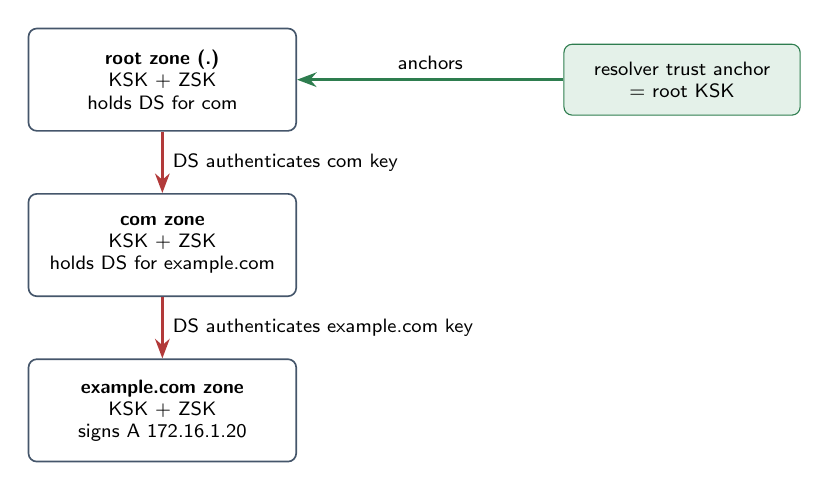
\begin{tikzpicture}[font=\sffamily\scriptsize,
  zz/.style={draw=dslate,rounded corners=3pt,fill=white,minimum width=34mm,minimum height=13mm,align=center,line width=0.6pt},
  ds/.style={->,>=Stealth,bad,line width=0.9pt},
  tabox/.style={draw=good,fill=goodlt,rounded corners=3pt,minimum width=30mm,minimum height=9mm,align=center}
]
\node[zz] (root) at (0,0) {\textbf{root zone (.)}\\KSK + ZSK\\holds DS for com};
\node[zz] (com) at (0,-2.1) {\textbf{com zone}\\KSK + ZSK\\holds DS for example.com};
\node[zz] (ex) at (0,-4.2) {\textbf{example.com zone}\\KSK + ZSK\\signs A 172.16.1.20};
\node[tabox] (ta) at (6.6,0) {resolver trust anchor\\= root KSK};
\draw[ds] (root.south) -- node[right,black]{DS authenticates com key} (com.north);
\draw[ds] (com.south) -- node[right,black]{DS authenticates example.com key} (ex.north);
\draw[->,>=Stealth,good,line width=0.9pt] (ta.west) -- node[above,black]{anchors}(root.east);
\end{tikzpicture}
\caption{The DNSSEC chain of trust. The resolver trusts only the root key signing key, and each parent's signed DS record authenticates the child's key, so trust flows from the root down to the example.com A record without the resolver needing to know any key but the anchor.}
\label{fig:p3-chain}
\end{figure}

The signing is done by \texttt{scripts/sign-zones.sh}, which for each of the three
zones generates a zone signing key and a key signing key with
\texttt{dnssec-keygen}, appends both public keys to the zone, and signs the zone
with \texttt{dnssec-signzone}. It then derives the child's DS record from its key
signing key with \texttt{dnssec-dsfromkey -2}, which uses SHA-256 for the digest,
and appends that DS into the parent zone before signing the parent. The order is
bottom up, that is \texttt{example.com} first, then \texttt{com} with
\texttt{example.com}'s DS, then the root with \texttt{com}'s DS, which is what
produces a consistent chain. Finally the script extracts the root key signing key
and writes it into the resolver's trust anchor file.

\begin{lstlisting}[language=bash,caption={The heart of the signing script, which generates keys, publishes the child DS in the parent, and signs bottom up (scripts/sign-zones.sh, abridged).}]
dnssec-keygen -a ECDSAP256SHA256 -n ZONE example.com        # ZSK
dnssec-keygen -a ECDSAP256SHA256 -f KSK -n ZONE example.com # KSK
dnssec-signzone -S -o example.com -f db.example.com.signed db.example.com.unsigned
dnssec-dsfromkey -2 Kexample.com.+013+XXXXX.key > dsset-example.com
# dsset-example.com is appended into com before com is signed; com's DS into root.
\end{lstlisting}

On the resolver side, validation is switched on with \texttt{dnssec-validation
yes} and the root key signing key is installed as the single trust anchor, while
the root hints are left pointing at the lab root server exactly as in Phase 1.

\begin{lstlisting}[language=,caption={The resolver's trust anchor, a static root KSK (configs/trust-anchors.conf).}]
trust-anchors {
    . static-key 257 3 13 "A+jYngeG3x3mfMvQKa3yfi41+fM/f9/Z/GapyPr+Ztd...==";
};
\end{lstlisting}

\textbf{Signing algorithm choice.} The zones are signed with ECDSA using the P-256
curve and SHA-256, which is algorithm 13. This is a deliberate choice. Compared
with RSA it produces much smaller keys and signatures for equivalent strength,
which keeps DNS responses compact and reduces the chance of fragmentation or
fallback to TCP, and it is widely supported by modern validating resolvers. Its
trade-off is that it is more sensitive to a sound source of randomness during
signing and is slightly more expensive to verify than to generate, though neither
matters at laboratory scale. The main practical cost is simply that very old
resolvers might not recognise the algorithm, which is not a concern here.

\subsection{Verifying a healthy signed hierarchy}

Before attacking, the signed hierarchy is checked with no interceptor on the path.
A \texttt{dig +dnssec example.com} returns the address together with its RRSIG and,
most importantly, with the \texttt{ad} flag set, which is the resolver's statement
that it validated the answer. An independent check with \texttt{delv}, pointed at
the lab root key as its trust anchor, reports the answer as fully validated.

\begin{lstlisting}[language=,caption={Healthy validation before the attack, showing the ad flag and a valid RRSIG, with delv reporting full validation (evidence/p3-valid-dig.txt, p3-valid-delv.txt).}]
;; flags: qr rd ra ad; QUERY: 1, ANSWER: 2, ...
example.com.  300  IN  A      172.16.1.20
example.com.  300  IN  RRSIG  A 13 2 300 20261122142217 20261023142217 25557 example.com. ...

; fully validated          <-- delv, anchored on the lab root key
\end{lstlisting}

\shot{Healthy DNSSEC validation. \texttt{dig +dnssec} shows the \texttt{ad} flag and a valid RRSIG, and \texttt{delv} reports the chain as fully validated against the root trust anchor.}{dig +dnssec output with the ad flag visible and the RRSIG present, and delv printing "fully validated"}{phase3/evidence/p3-valid-dig.txt, p3-valid-delv.txt}{fig:p3-valid}

The screenshot in Figure~\ref{fig:p3-valid} is the verification required by 3.2.
It should show the \texttt{ad} flag in the \texttt{dig} header and the RRSIG
accompanying the address, together with the \texttt{delv} line reporting full
validation. These are the signs that the signed hierarchy is healthy and that the
whole chain from the root down to \texttt{example.com} verifies, which is the
necessary starting point before the attack is re-run.

\subsection{Re-running the forgery under DNSSEC}

The Phase 2 attack is now re-run without modification, and the result is completely
different. The forged and unsigned answer carries no valid signature from the
\texttt{example.com} key, so the validating resolver refuses to accept it and fails
the lookup rather than caching a lie. It exhausts its attempts to obtain a signed
answer that it can validate and then returns SERVFAIL with an empty answer section,
which the capture below records. The client's web fetch therefore fails at the name
resolution step and never reaches the rogue server.

The cause of the failure is signature validation rather than any network fault. The
attacker holds no zone key, so the record it injects carries no RRSIG that the
resolver can verify against the \texttt{example.com} zone key, and a validating
resolver treats a signed zone whose data does not verify as bogus. The very packet
that poisoned the cache in Phase 2 is simply discarded here, which is the whole
difference that DNSSEC makes.

\begin{lstlisting}[language=,caption={The validating resolver returns SERVFAIL with an empty answer section for the forged answer (evidence/p3-attack-dig-servfail.txt).}]
;; ->>HEADER<<- opcode: QUERY, status: SERVFAIL, id: 5520
;; flags: qr rd ra; QUERY: 1, ANSWER: 0, AUTHORITY: 0, ADDITIONAL: 1
;; QUESTION SECTION:
;example.com.			IN	A
;; Query time: 4 msec
;; SERVER: 172.16.2.10#53(172.16.2.10) (UDP)
\end{lstlisting}

\shot{The re-run attack under DNSSEC. The validating resolver rejects the forged answer and returns SERVFAIL with an empty answer section, and \texttt{curl} cannot resolve the host, so the client never reaches the rogue page.}{dig with +time=6 +tries=2 showing a SERVFAIL status and no answer, next to curl reporting "Could not resolve host"}{phase3/evidence/p3-attack-dig-servfail.txt, p3-attack-curl.txt}{fig:p3-attack}

The screenshot in Figure~\ref{fig:p3-attack} is the evidence for 3.3 and 3.4. It
should show the resolver failing the lookup with a SERVFAIL status rather than
returning the rogue address, and it should show the client's fetch failing to
resolve the host. Together they establish that the identical attack which succeeded
in Phase 2 no longer works once the resolver validates the chain, because the
forged record carries no signature the resolver can verify.

\subsection{Analysis and Discussion}

\textbf{What the resolver checks, and how this differs from Phase 2.} In Phase 2
the resolver accepted the first matching reply and cached 172.16.1.30. Here the
resolver requires that the address record be accompanied by an RRSIG that verifies
under the \texttt{example.com} zone key, that the zone key in turn be authenticated
by the DS record in \texttt{com}, and that the \texttt{com} key be authenticated by
the DS in the root, which is finally vouched for by the trust anchor the resolver
holds. The forged answer satisfies none of this, because the attacker holds no zone
key and cannot produce a valid signature, so the chain breaks and the resolver
returns failure instead of a poisoned record.

\textbf{What the attacker can still read, and what DNSSEC does and does not
protect.} Comparing the attacked exchange with the Phase 1 capture shows that
DNSSEC changed nothing about confidentiality. The query name, the transaction
identifier, the ports, and the answers are all still in cleartext on the wire, and
the on-path attacker can read every one of them exactly as before. What DNSSEC adds
is integrity and origin authentication of the data. The attacker can still see and
still inject, but it can no longer make the resolver believe a forged record,
because it cannot forge the signature. DNSSEC protects the authenticity of DNS
data, and it does not provide any privacy for it.

\textbf{Whether any private key belongs in the repository.} No. The private
components of the key signing and zone signing keys are exactly what an attacker
would need in order to forge valid signatures and defeat the entire chain, so they
must never be committed. The repository carries the signing scripts and the public
material needed to reproduce a signed hierarchy, and the keys themselves are
regenerated on a clean checkout rather than shipped.

\takeaway{\textbf{Outcome.} The attack is blocked. DNSSEC authenticates the data, so the plain forgery that worked in Phase 2 now fails. The resolver detects the missing signature and refuses the answer. The attacker can still read everything on the wire, since DNSSEC adds no confidentiality.}

\clearpage

% =====================================================================
% PHASE 4
% =====================================================================
\section{Signature Stripping and Downgrade (Phase 4)}

\subsection{Objective}

Since a forged signed answer failed in Phase 3, Phase 4 asks the obvious next
question. Rather than forge a signature, can the attacker make the signed zone
appear to be unsigned, so that the resolver stops expecting signatures and the
plain forgery is accepted again? The attacker is allowed to rewrite anything in
transit but still holds no private keys. The phase is run in two contrasting
configurations, and the contrast between them is the entire lesson.

\subsection{Design and implementation}

The interceptor is extended into a stripper, in \texttt{src/stripper.c}, with
three modes selected on the command line. The relay mode is the transparent relay
used for verification. The two strip modes both forge the final
\texttt{example.com} A answer, but they differ in how much of the DNSSEC material
around it they remove.

In \texttt{--strip-runA}, the stripper removes every DNSSEC-related record type,
namely RRSIG, DNSKEY, DS, NSEC, NSEC3, NSEC3PARAM, CDS, and CDNSKEY, from all
sections of every response it relays. This is the fuller downgrade, because it
removes not only the signatures on the \texttt{example.com} answer but also the DS
record, and its RRSIG, from the \texttt{com} referral, which is the attacker's
attempt to hide the fact that the child is supposed to be secure. In
\texttt{--strip-runB}, the stripper forges the same \texttt{example.com} A answer
but leaves the parent's records untouched. The attacker discovers the resolver's
hardware address by ARP at start-up and detects its interface by address, so the
behaviour does not depend on hard-coded values.

The two runs also differ in the deployment. Run A uses the unchanged Phase 3
hierarchy, in which \texttt{com} publishes a DS for \texttt{example.com}. Run B
re-signs \texttt{com} with \texttt{scripts/sign-zones-runB.sh} so that it publishes
no DS for \texttt{example.com}, while \texttt{example.com} itself stays fully
signed and the root and the trust anchor are untouched. This single change models a
specific and realistic operator error.

\subsection{Verification}

Before stripping, the client still resolves \texttt{example.com} as an
authenticated answer through the transparent relay, with the \texttt{ad} flag set
and the real address returned. This confirms that the starting point for both runs
is a healthy, validated resolution and that the stripper in relay mode changes
nothing.

\shot{Verification before stripping. Through the transparent relay the client still resolves \texttt{example.com} to 172.16.1.20 with the \texttt{ad} flag set and fetches the real page.}{dig +dnssec through the relay showing ad and 172.16.1.20, and curl returning the real page}{phase4/evidence/a-verify-dig.txt, a-verify-curl.html}{fig:p4-verify}

The screenshot in Figure~\ref{fig:p4-verify} is the verification required by 4.2.
It should show the authenticated answer and the real page while the stripper is on
the path in relay mode, which establishes that anything different seen in the two
attack runs is caused by stripping and forging, not by the attacker's presence.

\subsection{Run A, stripping against the full chain}

In Run A the stripper removes every \texttt{example.com}-scoped DNSSEC record on
the wire and injects the forged address, and its own log confirms that it did so.
The resolver, however, returns SERVFAIL, and the fetch fails.

\begin{lstlisting}[language=,caption={Run A result: the strip-and-forge attack fails (evidence/a-attack-dig.txt).}]
;; ->>HEADER<<- opcode: QUERY, status: SERVFAIL, id: 8968
;; flags: qr rd ra; QUERY: 1, ANSWER: 0, ...
\end{lstlisting}

The reason is the most important idea in the phase. Because \texttt{com} publishes
a DS for \texttt{example.com}, the resolver has already learned, from authenticated
data, that \texttt{example.com} is supposed to be secure. A validating resolver
only treats a delegation as insecure when it holds an authenticated proof that no
DS exists, namely a signed denial from the parent. The on-path attacker holds no
\texttt{com} key, so it can neither forge that proof nor strip its way to one.
Removing the signatures does not make the zone look unsigned. It makes the zone
look broken, and broken resolves to SERVFAIL rather than to a cached forgery. The
resolver's log naming a broken trust chain is the direct evidence of this.

\shot{Run A evidence. The stripper log shows the DNSSEC records removed and the A record forged, yet the resolver reports a broken trust chain and returns SERVFAIL.}{the stripper-runA.log [STRIP] and [FORGE] lines, the SERVFAIL dig, and the resolver "broken trust chain" log line, shown together}{phase4/evidence/stripper-runA.log, a-attack-dig.txt, a-resolver-log.txt}{fig:p4-runA}

The screenshot in Figure~\ref{fig:p4-runA} is the Run A evidence for 4.3 and 4.4.
It should show that the attacker genuinely stripped and forged, from its own log,
and that the resolver nonetheless refused the result with a broken trust chain.
The pairing matters, because it proves the failure is the resolver detecting an
unverifiable delegation, not the attack failing to execute.

\subsection{Run B, the operator mistake}

Run B changes one thing in the deployment: \texttt{com} is re-signed so that it no
longer publishes \texttt{example.com}'s DS, while \texttt{example.com} itself stays
fully signed and the root and the trust anchor are untouched. The attacker performs
the same core strip-and-forge of the \texttt{example.com} answer as in Run A, but it
now leaves the parent's records in place rather than stripping them. The reason is
specific. In this deployment \texttt{com}'s own signed denial authenticatedly proves
that \texttt{example.com} has no DS, and that genuine, signed proof is exactly what
the attack needs the resolver to receive, so stripping it away would defeat the
attack rather than help it. With that proof delivered, the root-anchored resolver
concludes that the delegation is insecure, stops validating the child, and accepts
the unsigned forged answer.

\begin{lstlisting}[language=,caption={Run B: delv reports an insecure (unsigned) delegation, and the forged answer is accepted with no ad flag (evidence/b-delv-insecure.txt, b-attack-dig.txt).}]
; unsigned answer                 <-- delv: no secure link into example.com
example.com.  300  IN  A  172.16.1.20

;; ->>HEADER<<- opcode: QUERY, status: NOERROR, id: 26383   (note: NO ad flag)
example.com.  300  IN  A  172.16.1.30     <-- forged, accepted
\end{lstlisting}

The decisive detail is that the Run B answer carries no \texttt{ad} flag. The
resolver is not claiming the answer is authenticated. It has correctly determined
that the zone is insecure and is behaving exactly as the standard requires for an
insecure zone, which is to pass the answer through unvalidated. The failure is not
in the resolver's logic. It is in the delegation, which never had a secure link
into it. Figure~\ref{fig:p4-decision} shows the two paths side by side.

\shot{Run B evidence. With no DS in the parent, the delegation is authenticated as insecure, and the same strip-and-forge attack now lands the client on the rogue page at 172.16.1.30.}{delv reporting "unsigned answer", the no-DS signed denial, dig returning 172.16.1.30 with no ad flag, and the rogue page}{phase4/evidence/b-delv-insecure.txt, b-ds-nodata.txt, b-attack-dig.txt, b-attack-curl.html}{fig:p4-runB}

The screenshot in Figure~\ref{fig:p4-runB} is the Run B evidence for 4.3 and 4.4.
It should show that the delegation is now authenticated as insecure, from the
\texttt{delv} output and the signed no-DS denial, and that the forged address is
consequently accepted and the rogue page loads. The absence of the \texttt{ad}
flag on the accepted answer is the detail to mark, because it shows the resolver
is treating the zone as insecure rather than claiming to have validated a lie.

\begin{figure}[H]
\centering
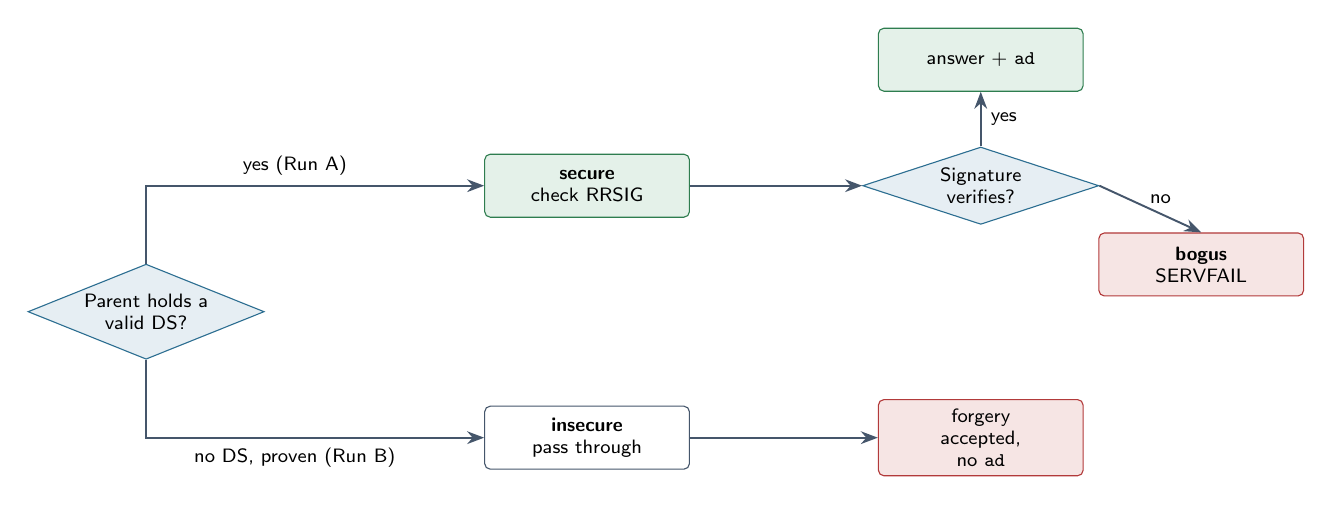
\begin{tikzpicture}[font=\sffamily\scriptsize,
  dec/.style={draw=accent,fill=accentlt,diamond,aspect=2.4,align=center,inner sep=1pt,minimum width=30mm},
  res/.style={rounded corners=2pt,minimum width=26mm,minimum height=8mm,align=center},
  a/.style={->,>=Stealth,dslate,line width=0.7pt}
]
\node[dec] (q) at (0,0) {Parent holds a\\valid DS?};
\node[res,draw=good,fill=goodlt] (secure) at (5.6,1.6) {\textbf{secure}\\check RRSIG};
\node[res,draw=dslate,fill=white] (insecure) at (5.6,-1.6) {\textbf{insecure}\\pass through};
\node[dec] (q2) at (10.6,1.6) {Signature\\verifies?};
\node[res,draw=good,fill=goodlt] (ok) at (10.6,3.2) {answer + \texttt{ad}};
\node[res,draw=bad,fill=badlt] (bogus) at (13.4,0.6) {\textbf{bogus}\\SERVFAIL};
\node[res,draw=bad,fill=badlt] (acc) at (10.6,-1.6) {forgery\\accepted,\\no \texttt{ad}};
\draw[a] (q.north) |- node[above,black,pos=0.72]{yes (Run A)} (secure.west);
\draw[a] (q.south) |- node[below,black,pos=0.72]{no DS, proven (Run B)} (insecure.west);
\draw[a] (secure.east) -- (q2.west);
\draw[a] (q2.north) -- node[right,black]{yes} (ok.south);
\draw[a] (q2.east) -- node[above,black,pos=0.6]{no} (bogus.north);
\draw[a] (insecure.east) -- (acc.west);
\end{tikzpicture}
\caption{The resolver's delegation decision. Run A follows the upper path to bogus because a DS exists but the stripped answer no longer verifies. Run B follows the lower path to insecure because the parent authenticatedly proves no DS exists, and the forgery is then accepted.}
\label{fig:p4-decision}
\end{figure}

\subsection{Analysis and Discussion}

\textbf{Run A, why the attacker cannot make the zone look unsigned.} Stripping
signatures off the wire does not remove the parent's knowledge that the child is
secure. The DS in \texttt{com} is authenticated and the attacker cannot touch it
without a \texttt{com} key, so the resolver still demands a valid signature it
cannot be given, and the result is bogus rather than insecure. A side effect worth
noting is that stripping also makes names below the zone, such as \texttt{www},
fail while the attack runs, because the whole zone becomes unvalidatable. That is
the true consequence of a zone-wide downgrade attempt, not a working partial
attack.

\textbf{Run B, the change that reopens the attack.} The one change to the deployment
is that \texttt{com} no longer publishes \texttt{example.com}'s DS, and that is what
reopens the forgery. The core strip-and-forge of the \texttt{example.com} answer is
deliberately the same in both runs. The only difference in the attacker's behaviour
is that Run A additionally strips the parent's DS on the wire, which is exactly the
fuller downgrade the task calls for and exactly what is shown to be futile. That the
decisive factor is the parent's DS, and not how hard the attacker strips, is clear
from the contrast. Run A fails even though it strips more, and Run B succeeds even
though it strips less. The missing DS turns the parent's signed denial of a DS into
an authenticated statement that the child is insecure, which tells the resolver to
stop validating it. To a validating resolver, a fully signed zone whose DS was never
published in its parent is indistinguishable from an unsigned zone.

\textbf{Where downgrade resistance comes from.} It comes from the parent side,
specifically from the signed DS record and the signed denial of a DS, not from the
child's own signatures. The exact operator mistake that forfeits it is signing a
zone but never publishing, or allowing to lapse, its DS in the parent. The child
can be perfectly signed and still be wide open, because the security of a
delegation is decided one level up.

\takeaway{\textbf{Outcome.} Run A is blocked and Run B succeeds. The core strip-and-forge is the same in both, and the decisive difference is a missing DS record in the parent, shown by the fact that Run A fails while stripping more and Run B succeeds while stripping less. Downgrade resistance is a property of the parent's delegation, and an operator who signs a zone without wiring up its DS has a zone that is signed in name only.}

\clearpage

% =====================================================================
% PHASE 5
% =====================================================================
\section{Zone Walking (Phase 5)}

\subsection{Objective}

Phase 5 turns from forging answers to a subtler problem, which is the information a
signed zone leaks about itself simply by being able to prove that a name does not
exist. Authenticated denial has to be signed ahead of time, before anyone knows
which nonexistent name will be queried, because the server cannot mint a fresh
signature per query without keeping its private key online. A proof prepared in
advance cannot be about the queried name, so it must instead speak about the names
that do exist, and that is the leak the phase exploits and then closes.

\subsection{Design and implementation}

The \texttt{example.com} zone is populated with five unadvertised internal
hostnames, \texttt{backup}, \texttt{dev}, \texttt{git}, \texttt{mail}, and
\texttt{vpn}, alongside the public \texttt{www} and \texttt{ns}. None of the five
is referenced anywhere a client would normally learn it, so recovering them is a
genuine disclosure. The deployment is otherwise the Phase 3 signed, validating
hierarchy. The zone is first signed with NSEC for authenticated denial, using
\texttt{scripts/sign-zones.sh}, and later re-signed with NSEC3 as the fix, using
\texttt{scripts/sign-zones-nsec3.sh}.

The attacker on the resolver subnet runs a C and \texttt{libpcap} walker, in
\texttt{src/walker.c}. It injects a query for a name's NSEC record with the DNSSEC
OK bit set, from a source UDP port the kernel is not using so the reply is not
intercepted by the host stack, reads the signed denial off the wire, and takes the
next owner name from the NSEC record. It then queries that name's NSEC, and
repeats, until a record's next-name wraps back to the apex. No zone transfer and no
wordlist are used. Against an NSEC3-signed zone the apex carries no NSEC record, so
the first step finds no next-name and the walk recovers nothing.

\begin{figure}[H]
\centering
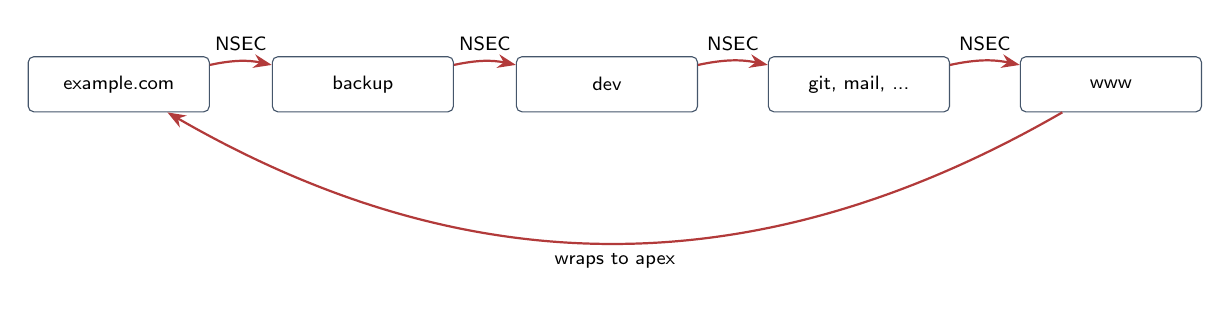
\begin{tikzpicture}[font=\sffamily\scriptsize,
  n/.style={draw=dslate,rounded corners=2pt,fill=white,minimum width=23mm,minimum height=7mm,align=center},
  a/.style={->,>=Stealth,bad,line width=0.8pt,bend left=12}
]
\node[n] (apex) at (0,0) {example.com};
\node[n] (backup) at (3.1,0) {backup};
\node[n] (dev) at (6.2,0) {dev};
\node[n] (etc) at (9.4,0) {git, mail, ...};
\node[n] (www) at (12.6,0) {www};
\draw[a] (apex) to node[above,black]{NSEC} (backup);
\draw[a] (backup) to node[above,black]{NSEC} (dev);
\draw[a] (dev) to node[above,black]{NSEC} (etc);
\draw[a] (etc) to node[above,black]{NSEC} (www);
\draw[->,>=Stealth,bad,line width=0.8pt,bend left=30] (www) to node[below,black]{wraps to apex} (apex);
\end{tikzpicture}
\caption{The NSEC chain. Each record names its successor in canonical order and in cleartext, so a denial for any name hands the attacker the next real name. Following the chain from the apex visits every owner and wraps back to the start.}
\label{fig:p5-nsec}
\end{figure}

\subsection{Verifying how a signed zone denies a name}

A query for a name that does not exist returns NXDOMAIN, but under NSEC that denial
comes with a signed NSEC record whose owner and next-name span the queried name.
That record is a signed statement that nothing exists between one real name and the
next real name, which means it discloses a real neighbouring name as a side effect
of proving the absence of the queried one.

\shot{A signed NSEC denial for a nonexistent name. The NXDOMAIN response carries an NSEC record and its RRSIG whose span discloses a real neighbouring name.}{dig +dnssec for a nonexistent name showing NXDOMAIN with the NSEC record and RRSIG in the authority section}{phase5/evidence/p5-nxdomain.txt}{fig:p5-nxdomain}

The screenshot in Figure~\ref{fig:p5-nxdomain} is the verification required by 5.2.
It should show the signed NXDOMAIN response and, within it, the NSEC record whose
owner and next-name bracket the queried name. The point to notice is that the
proof of nonexistence necessarily names a real neighbour, which is the exact
property the walk exploits.

\subsection{Walking the zone}

Starting from knowledge of \texttt{example.com} alone, the walker follows the NSEC
chain and recovers all eight owner names in eight queries, which is within the
budget of the number of names plus two. Every one of the five hidden internal
hosts is exposed.

\begin{lstlisting}[language=,caption={The full NSEC walk, recovering every name including the five hidden hosts (evidence/p5-walk-nsec.txt).}]
found: example.com         next -> backup.example.com
found: backup.example.com  next -> dev.example.com
found: dev.example.com     next -> git.example.com
found: git.example.com     next -> mail.example.com
found: mail.example.com    next -> ns.example.com
found: ns.example.com      next -> vpn.example.com
found: vpn.example.com     next -> www.example.com
found: www.example.com     next -> example.com
recovered 8 owner name(s) in 8 queries
\end{lstlisting}

\shot{The complete NSEC walk. The walker follows the chain from the apex and recovers all eight owner names, including backup, dev, git, mail, and vpn, in eight queries.}{the walker output listing all recovered names and "chain wrapped to apex"}{phase5/evidence/p5-walk-nsec.txt}{fig:p5-walk}

The screenshot in Figure~\ref{fig:p5-walk} is the central evidence for 5.3. It
should show the walker stepping through the chain and the final list of recovered
names, including the five that were never advertised. The query count, one per
name, confirms that the recovery stayed within the stated budget and used ordinary
DNS queries rather than a transfer or a guess list.

\subsection{Closing the leak with NSEC3}

The fix is to re-sign \texttt{example.com} with NSEC3, which chains hashes of the
owner names rather than the names themselves. A nonexistent name still receives a
valid, signed denial, so the security property is preserved. This is confirmed
independently of the walk. A query for a nonexistent name under NSEC3 still returns
an NXDOMAIN status with the \texttt{ad} flag set and signed NSEC3 records in the
authority section, which is the resolver's statement that the denial itself
validated. The difference is that the denial now reveals only a hash and not a
cleartext neighbour. When the walk is re-run, the apex query returns no usable
next-name, and the walker recovers nothing. The two facts together, an authenticated
denial that still validates and a walk that now fails, show the fix is both sound and
effective.

\begin{lstlisting}[language=,caption={After the NSEC3 fix the same walk recovers nothing (evidence/p5-walk-nsec3.txt).}]
example.com: signed denial carries NO NSEC next-name (NSEC3 ...) -> walk cannot continue
recovered 0 owner name(s) in 1 queries
\end{lstlisting}

\shot{After the NSEC3 fix. A nonexistent name still gets an authenticated denial, now via hashed NSEC3 records, and the re-run walk recovers zero names.}{p5-nxdomain-nsec3 showing the hashed NSEC3 denial, and p5-walk-nsec3 showing the walk failing with 0 names}{phase5/evidence/p5-nxdomain-nsec3.txt, p5-walk-nsec3.txt}{fig:p5-nsec3}

The screenshot in Figure~\ref{fig:p5-nsec3} is the evidence that the fix works,
required by 5.3. It should show two things. The first is that a nonexistent name
still receives a valid signed denial, now carrying hashed NSEC3 records instead of
cleartext names. The second is that the same walker now recovers nothing. The
combination proves the fix preserves authenticated denial while removing the
enumeration it previously enabled.

\subsection{Analysis and Discussion}

\textbf{Names recovered and the exact steps.} The walk recovered \texttt{backup},
\texttt{dev}, \texttt{git}, \texttt{mail}, and \texttt{vpn}, together with
\texttt{www}, \texttt{ns}, and the apex. The procedure is one query per name. The
walker asks for a name's NSEC with the DNSSEC OK bit set, reads the next name from
the record, and queries that, continuing until the next-name wraps to the apex.
Eight names came out in eight queries.

\textbf{Which configuration made the walk possible, and why signed denial leaks
when plain DNS does not.} NSEC made it possible. Because authenticated denial must
be pre-signed, the proof cannot concern the queried name and must instead point at
names that do exist, in canonical order, and NSEC publishes those successor names
in cleartext. Each denial is therefore a signed statement naming a real neighbour.
Plain unsigned DNS simply returns NXDOMAIN with no such span, so it reveals nothing
about any other name.

\textbf{What the fix costs and what an enumerator can still learn.} NSEC3 costs
extra CPU to hash, produces larger denials, and introduces salt and iteration
parameters, along with an opt-out option that weakens the guarantee if enabled. A
word on those parameters is warranted, because the intuition that more hashing means
more security is wrong here. Current best practice, set out in RFC 9276, is to use
zero extra iterations and an empty salt. Additional iterations add negligible
protection against offline cracking while multiplying the work the resolver and the
server must do for every query, which becomes a denial-of-service amplification
vector, and a per-zone salt does not help against an attacker who computes hashes on
demand. The zone in this lab was signed with a salt and ten iterations. That choice
still closes the walk, but it is a deliberate lab setting that departs from the
current recommendation rather than an improvement on it, and a production zone
should prefer zero iterations and no salt. Even with NSEC3 an enumerator can still
learn the number of names from the chain length, and it can attack the exposed
hashes offline with dictionaries or GPU brute force. NSEC3 therefore raises the cost
of enumeration without making it impossible. Removing even that residual leak
requires online signing schemes, at the price of keeping a private key online.

\takeaway{\textbf{Key observation.} Authenticated denial must be pre-signed, and a pre-signed proof about the gaps between names necessarily describes the names themselves. NSEC leaks them in cleartext, while NSEC3 replaces them with hashes, which is a large improvement but not a complete cure.}

\clearpage

% =====================================================================
% PHASE 6
% =====================================================================
\section{Last-Mile Response Forgery (Phase 6)}

\subsection{Objective}

The signed hierarchy and the validating resolver protect the data within the DNS,
but they do nothing for the final hop from the resolver to the client. A stub
resolver on the client does not validate signatures. It simply trusts whatever
appears to come from its resolver, including the \texttt{ad} flag that claims the
answer was authenticated. Phase 6 moves the adversary into the client subnet at
172.16.1.100 and forges the reply in exactly the place where DNSSEC's guarantee has
already run out, because validation happened one hop upstream and its result was
never carried down to the client in any verifiable form.

\subsection{Design and implementation}

The upstream hierarchy and the validating resolver are the unchanged Phase 3
deployment. The diversion this time is a route on the edge router that sends the
client-bound replies through the attacker, with no ARP spoofing and with the
client's own configuration untouched.

\begin{lstlisting}[language=bash,caption={The Phase 6 diversion on the edge router, detecting its interface by address (scripts/divert-on.sh).}]
DEV=$(ip -o -4 addr show | awk '/172\.16\.1\./{print $2; exit}')
ip route replace 172.16.1.10 via 172.16.1.100 dev "$DEV"
\end{lstlisting}

The attacker runs a C and \texttt{libpcap} forger, in \texttt{src/forge.c}, with a
relay mode and a forge mode. In forge mode, for the client-bound
\texttt{example.com} answer, it injects a reply pointing at the rogue server at
172.16.1.30, and it sets the \texttt{ad} flag in that forged reply. The attack is
run against two different clients so that the contrast makes the lesson clear.
Client A is an ordinary stub using the operating system resolver, and Client B is a
locally validating client using \texttt{delv} that holds the root key as its own
trust anchor. Figure~\ref{fig:p6-lastmile} shows where the forgery happens.

\begin{figure}[H]
\centering
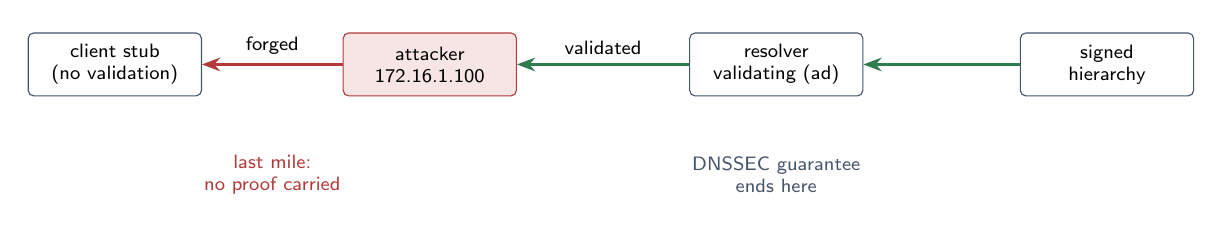
\begin{tikzpicture}[font=\sffamily\scriptsize,
  n/.style={draw=dslate,rounded corners=2pt,fill=white,minimum width=22mm,minimum height=8mm,align=center},
  atk/.style={draw=bad,fill=badlt,rounded corners=2pt,minimum width=22mm,minimum height=8mm,align=center},
  a/.style={->,>=Stealth,line width=0.8pt}
]
\node[n] (client) at (0,0) {client stub\\(no validation)};
\node[atk] (atk) at (4,0) {attacker\\172.16.1.100};
\node[n] (res) at (8.4,0) {resolver\\validating (ad)};
\node[n] (up) at (12.6,0) {signed\\hierarchy};
\draw[a,good] (up) -- (res);
\draw[a,good] (res) -- node[above,black]{validated} (atk);
\draw[a,bad] (atk) -- node[above,black]{forged} (client);
\node[dslate,align=center] at (8.4,-1.4) {DNSSEC guarantee\\ ends here};
\node[bad,align=center] at (2,-1.4) {last mile:\\ no proof carried};
\end{tikzpicture}
\caption{The last mile. DNSSEC validation happens at the resolver, but the resolver to client hop carries no proof of it, so an on-path attacker on that hop can replace the answer after validation is already behind it.}
\label{fig:p6-lastmile}
\end{figure}

\subsection{Verification}

With the attacker relaying transparently, the client still resolves
\texttt{example.com} and fetches the real page, which confirms the diversion itself
is harmless until forging is switched on.

\shot{Transparent relay on the last mile. With forging disabled, the client still resolves \texttt{example.com} to 172.16.1.20 and fetches the real page.}{dig showing 172.16.1.20 with the ad flag and curl returning the real page through the relay}{phase6/evidence/p6-verify-dig.txt, p6-verify-curl.html}{fig:p6-verify}

The screenshot in Figure~\ref{fig:p6-verify} is the verification required by 6.2.
It should show the client receiving the correct address and the genuine page while
the attacker relays, so that the two client outcomes that follow can be attributed
to the forgery rather than to the diversion.

\subsection{The attack}

Client A accepts the forged reply and loads the rogue page at 172.16.1.30, and the
forged reply even carries the \texttt{ad} flag, because the attacker set it. This
is the crux of the phase. A flag that is supposed to mean the answer was
authenticated is only a single unauthenticated bit that whoever writes the packet
can set at will.

\begin{lstlisting}[language=,caption={Client A, an ordinary stub, accepts the forged last-mile reply, ad flag and all (evidence/p6-clientA-dig.txt).}]
;; ->>HEADER<<- opcode: QUERY, status: NOERROR, id: 3468
;; flags: qr rd ra ad; QUERY: 1, ANSWER: 1, ...
example.com.  300  IN  A  172.16.1.30
\end{lstlisting}

Client B does something different. Because it validates the chain itself, anchored
on the root key it holds, it checks the signatures rather than trusting the flag,
finds that the forged A record has no valid RRSIG, and reports the answer as bogus,
returning no address. The forgery that fooled the stub is caught the moment
someone actually verifies the cryptography rather than believing a bit in a header.

\shot{Client A on the rogue page. The ordinary stub accepts the forged reply, with the \texttt{ad} flag set by the attacker, and \texttt{curl} returns the defacement page at 172.16.1.30.}{dig showing 172.16.1.30 with ad set, and curl returning the rogue page}{phase6/evidence/p6-clientA-dig.txt, p6-clientA-curl.html}{fig:p6-clientA}

The screenshot in Figure~\ref{fig:p6-clientA} is the Client A evidence for 6.3. It
should show the stub accepting the rogue address with the \texttt{ad} flag present,
and the rogue page loading. The presence of the \texttt{ad} flag on a forged answer
is the detail that proves the flag carries no real guarantee on the last mile.

\shot{Client B catches the forgery. The locally validating client checks signatures itself and reports the forged answer as bogus, returning no address.}{delv output reporting the answer as bogus or "insecurity proof failed" and refusing to return an address, captured with 2>&1 since delv prints it to standard error}{phase6/evidence/p6-clientB-delv.txt}{fig:p6-clientB}

The screenshot in Figure~\ref{fig:p6-clientB} is the Client B evidence for 6.3 and
6.4. It should show \texttt{delv} rejecting the forged answer as bogus and
returning no address, which demonstrates that a client that performs its own
validation is not fooled by the forged \texttt{ad} flag. One practical note applies
here. The \texttt{delv} command writes its validation failure to standard error, so
it is run with \texttt{2>\&1}, and the submitted \texttt{p6-clientB-delv.txt}
accordingly records the ``insecurity proof failed'' rejection in full.

\subsection{Analysis and Discussion}

\textbf{Why DNSSEC does not stop this.} The distinction the phase draws out is
between where validation happens and where trust is placed. Validation happened at
the resolver. The stub places its trust not in any signature but in the channel to
the resolver and in the \texttt{ad} bit, and on the last mile that channel is
exactly what the attacker controls. DNSSEC protects data inside the DNS, and it does
not authenticate the resolver to stub link, so the upstream validation result never
protects a stub that cannot check it.

\textbf{What tells a stub its answer was validated, and why the attacker can set
it.} The only in-band signal is the \texttt{ad} flag in the reply header. That bit
is not meaningless in general. It is the resolver's honest statement that it
validated the data, and it is worth trusting precisely when the stub reaches the
resolver over a channel that is itself authenticated and secured. What it is not is
a cryptographic proof that travels with the answer. It carries no signature of its
own, so a non-validating stub cannot verify it and has no choice but to trust
whoever appears to be its resolver and the channel that carries the bit. On an
unprotected last mile that is exactly what the attacker controls, so the forged
reply simply asserts \texttt{ad} and the stub believes a forged answer was
authenticated. Client B does not rely on the bit at all. It performs validation
locally against its own trust anchor, and the missing signature gives the forgery
away. The remedy for the last mile is therefore either local validation on the
client, as Client B shows, or an authenticated and encrypted channel from the
client to the resolver.

\takeaway{\textbf{Outcome.} Client A is fooled and Client B is protected. The ordinary stub lands on the rogue page because it trusts a flag that anyone on the path can set. Validation that happens upstream protects nobody downstream unless the downstream party either validates for itself or is given an authenticated channel.}

\clearpage

% =====================================================================
% PHASE 7
% =====================================================================
\section{Encrypting the Last Mile with DoT and DoH (Phase 7)}

\subsection{Objective}

Phase 7 closes the last-mile gap by authenticating and encrypting the client to
resolver link, and then mounts the last-mile attack again from three different
angles to see what the encryption actually prevents. Because the attack of Phase 6
relied on the last mile carrying its answer in cleartext with no proof of the
resolver's identity, the defence provides exactly those two things, confidentiality
and authentication of the channel, and the phase measures how much that is worth.

\subsection{Design and implementation}

A private certificate authority is created with \texttt{scripts/make-pki.sh} and
installed in the client's trust store, with no insecure bypass permitted. The
script generates an elliptic-curve CA, then issues the resolver a certificate whose
subject alternative name is exactly \texttt{resolver.cs6008.local} and which carries
no IP entry, so that the client must connect by name and validates the certificate
against that hostname. For the impersonation attack the script also issues a second
certificate for the same name signed by a separate, untrusted CA, which stands in
for an attacker who can present a certificate but cannot get it signed by the lab
CA.

\begin{lstlisting}[language=bash,caption={The resolver certificate is issued for the hostname only, with no IP SAN (scripts/make-pki.sh, abridged).}]
openssl ecparam -name prime256v1 -genkey -noout -out resolver.key
# extension file:  subjectAltName=DNS:resolver.cs6008.local   (no IP SAN)
openssl x509 -req -in resolver.csr -CA ca.crt -CAkey ca.key -CAcreateserial \
    -sha256 -extfile resolver.ext -out resolver.crt
cat resolver.crt ca.crt > resolver.fullchain.crt
\end{lstlisting}

The client reaches the resolver by name through a Compose \texttt{extra\_hosts}
entry that maps \texttt{resolver.cs6008.local} to the resolver address. The
resolver speaks DNS over TLS on TCP 853 and DNS over HTTPS on TCP 443, both backed
by the lab certificate, configured with a \texttt{tls} statement that names the key
and the full chain.

\begin{lstlisting}[language=,caption={The resolver's encrypted transports, both using the lab certificate (configs/resolver.conf, abridged).}]
tls lab-tls {
    key-file  "/lab/pki/resolver.key";
    cert-file "/lab/pki/resolver.fullchain.crt";
};
listen-on port 853 tls lab-tls { any; };               // DoT
listen-on port 443 tls lab-tls http default { any; };  // DoH at /dns-query
\end{lstlisting}

The upstream signed hierarchy is unchanged from Phase 3, and the attacker remains
on the client subnet as in Phase 6. Two client policies are tested against every
attack. The strict client, \texttt{scripts/resolve-strict.sh}, uses DoT only and
refuses any cleartext fallback. The permissive client,
\texttt{scripts/resolve-permissive.sh}, tries DoT first and falls back to cleartext
on any failure. This single policy difference decides every result in the phase.

The attacker uses a C and \texttt{libpcap} tool, \texttt{src/mitm.c}, together with
transport-layer attacks on the edge router. In \texttt{--forge-cleartext} it
rewrites the cleartext UDP port 53 \texttt{example.com} answer to the rogue address,
which is the Phase 6 forgery applied to any cleartext fallback. In
\texttt{--break-dot} it corrupts one payload byte of each DoT segment on TCP port
853, which makes the TLS integrity check fail and the session tear down. It cannot
read or forge the encrypted content, only break it. The rogue-certificate attempt
redirects port 853 to an OpenSSL server presenting the untrusted certificate, and
the transport-denial attempt blocks TCP 853 and 443 with \texttt{iptables}.

\subsection{Verifying an encrypted, authenticated last mile}

With no attacker on the path, the strict client resolves \texttt{example.com} over
DoT, the certificate validates cleanly against the lab CA and the hostname, the
upstream DNSSEC \texttt{ad} flag still holds, and a capture of the client's last
mile on the edge router shows no cleartext DNS at all, because the lookup went
entirely over TCP 853.

\begin{lstlisting}[language=,caption={Clean encrypted resolution over DoT, TLS 1.3, with the certificate validating against the lab CA (evidence/p7-verify-strict.txt).}]
[strict] DoT @resolver.cs6008.local (validating cert against lab CA)...
;; TLS session (TLS1.3)-(ECDHE-SECP256R1)-(ECDSA-SECP256R1-SHA256)-(AES-256-GCM)
;; Flags: qr rd ra ad; ...
example.com.  300  IN  A  172.16.1.20
\end{lstlisting}

\shot{Verified encrypted resolution. The strict client resolves over DoT with the certificate validating cleanly, the upstream \texttt{ad} flag intact, and a port-53 read of the capture showing no cleartext DNS on the last mile.}{p7-verify-strict showing the TLS1.3 session and 172.16.1.20, alongside the empty port-53 read of the capture}{phase7/evidence/p7-verify-strict.txt, p7-verify-no-cleartext.txt, p7-verify.pcap}{fig:p7-verify}

The screenshot in Figure~\ref{fig:p7-verify} is the verification required by 7.2.
It should show the encrypted DoT session establishing with a validated
certificate and returning the correct address, and it should show that a read of
the captured traffic filtered to port 53 is empty for the lookup. The empty
port-53 read is the positive evidence that no cleartext DNS crossed the last mile,
which is exactly what the encryption is meant to guarantee.

\subsection{Three attempts against two clients}

Three distinct attempts are mounted. Attempt (i) alters the answer in transit, by
corrupting the DoT stream and forging the cleartext fallback. Attempt (ii)
impersonates the resolver with a rogue certificate. Attempt (iii) denies the
encrypted transport outright by blocking TCP 853 and 443 to force a cleartext
fallback. Each is run against both clients, giving six outcomes, summarised in
Table~\ref{tab:p7-matrix}.

\begin{table}[H]
\centering
\small
\begin{tabularx}{\linewidth}{l Y Y}
\toprule
\textbf{Attempt} & \textbf{Strict client (refuses cleartext)} & \textbf{Permissive client (allows fallback)} \\
\midrule
(i) alter in transit &
\textbf{Blocked.} TLS integrity aborts the session, no answer &
\textbf{Lands.} Falls back to cleartext, forged to rogue \\
(ii) rogue certificate &
\textbf{Blocked.} Cert fails to chain to the lab CA, no answer &
\textbf{Lands.} DoT fails, falls back, forged to rogue \\
(iii) deny transport &
\textbf{Blocked.} No DoT, refuses cleartext, no answer &
\textbf{Lands.} Falls back to cleartext, forged to rogue \\
\bottomrule
\end{tabularx}
\caption{All six outcomes. The strict client defeats every attempt, while the permissive client falls to all three, and in every case the attacker won by denying DoT rather than by breaking it.}
\label{tab:p7-matrix}
\end{table}

The pattern in Table~\ref{tab:p7-matrix} is the whole result. Against the strict
client no attempt lands, because TLS gives the last mile confidentiality, so the
attacker cannot read the query to know what to forge, as well as integrity and
authentication, so it cannot alter the bytes and a rogue certificate fails to chain
to the lab CA or match the hostname. The most the attacker achieves against the
strict client is denial, and the strict client treats denial as failure rather
than dropping to cleartext.

Against the permissive client every attempt lands, but not by breaking the
cryptography. Each attempt merely denies DoT, whether by corrupting it, by
presenting a certificate the client rejects, or by blocking the port, and the
client's own willingness to fall back to cleartext then hands the answer to the
forger. The vulnerability is the fallback policy, not the encryption.

\begin{lstlisting}[language=,caption={The permissive client's fallback is the whole weakness, because DoT is denied, it drops to cleartext, and the forged 172.16.1.30 is accepted (evidence/p7-iii-permissive.txt).}]
[permissive] trying DoT @resolver.cs6008.local...
;; WARNING: can't connect to 172.16.2.10@853(TCP)
;; ERROR: failed to query server resolver.cs6008.local@853(TCP)
[permissive] DoT failed -> FALLING BACK TO CLEARTEXT (insecure).
example.com.  300  IN  A  172.16.1.30
\end{lstlisting}

\shot{All six outcomes under attack. For each of the three attempts, the strict client refuses cleartext and returns no answer, while the permissive client falls back and lands on the rogue address. Every strict run prints ``refusing cleartext; NO answer'', confirming it never downgrades.}{the six files side by side, with p7-i/ii/iii-strict each showing "refusing cleartext; NO answer", and p7-i/ii/iii-permissive each falling back to 172.16.1.30}{phase7/evidence/p7-i-strict.txt, p7-i-permissive.txt, p7-ii-strict.txt, p7-ii-permissive.txt, p7-iii-strict.txt, p7-iii-permissive.txt}{fig:p7-attacks}

The screenshot in Figure~\ref{fig:p7-attacks} is the attack evidence for 7.3, and
it covers all six attempt-by-client combinations rather than a representative few.
For each of the three attempts it should show the strict client refusing to fall
back and returning no answer, next to the permissive client falling back to
cleartext and accepting the forged address. Two things are worth confirming in it.
The first is that every one of the three strict runs prints ``refusing cleartext;
NO answer'', so the strict client never downgrades under any attempt. The second is
that every permissive run ends in the forged 172.16.1.30. The side-by-side
comparison is the proof that
every success against the permissive client came through the fallback and not
through any break of TLS.

\subsection{Analysis and Discussion}

\textbf{Every attempt and client, and why.} Against the strict client,
confidentiality denies the attacker the query it would need to forge, integrity
aborts any altered session, and certificate validation rejects the rogue identity,
so attempts (i) and (ii) fail outright and attempt (iii) achieves only a denial
that the strict policy treats as failure. Against the permissive client, all three
attempts succeed, but each does so only by denying DoT and relying on the client to
fall back to an unprotected channel, where the forger finishes the job.

\textbf{DoT or DoH, and the trade-off.} The client transport deployed here is DoT
on TCP 853, with DoH on 443 also enabled on the resolver. DoT's drawback relative
to DoH is precisely what attempt (iii) exploits. It uses a dedicated well-known
port, so a network operator or an on-path adversary can identify and block it
trivially, which is what forces the fallback. DoH hides DNS inside ordinary HTTPS
on 443, so it is harder to classify and block selectively, although it is not immune
to blocking, because an operator can still deny access to the known resolver
endpoint or its address. Its cost is that it is harder for a site operator to
monitor or filter, it carries a heavier HTTP stack, and it tends toward
centralisation in browsers. Neither transport changes the integrity or
authentication story, and they differ mainly in how selectively they can be blocked
and in operational visibility.

\textbf{What an encrypted, authenticated last mile still does not protect.} It
secures only the stub to resolver channel. It does not make an unsigned or
downgraded zone trustworthy, which remains the job of DNSSEC and correct
delegation. It does not help against a resolver that itself lies or is compromised.
It does not hide metadata such as the fact and timing of DNS activity, destination
addresses, or TLS size and server-name side channels. And it does nothing for a
client that accepts cleartext fallback or skips certificate validation, as the
permissive column shows in full. Confidentiality and last-mile integrity are
necessary but not sufficient, and end-to-end trust still needs DNSSEC validation,
ideally on the client, together with a firm no-downgrade policy.

\takeaway{\textbf{Outcome.} The strict client is immune and the permissive client falls. An authenticated, encrypted last mile defeats every last-mile attack for a client that refuses to downgrade. The one thing it cannot fix is a client that agrees to fall back to cleartext, because then the attacker never has to beat the cryptography at all. It simply switches it off.}

\clearpage

% =====================================================================
% CONCLUSION
% =====================================================================
\section{Synthesis and Conclusions}

Read as a whole, the seven phases tell a single coherent story about where trust
lives in DNS and what it takes to place it on firm ground. The plain hierarchy of
Phase 1 trusted the wire, and Phase 2 showed how cheaply that trust is betrayed by
anyone the topology puts on the path. Each later phase then moved the boundary of
trust and measured what the move bought.

The clearest lesson is that the two families of defence solve genuinely different
problems and neither substitutes for the other. DNSSEC, added in Phase 3 and probed
in Phases 4 and 5, authenticates DNS data. It proves that an answer came from the
zone that owns the name and was not altered, and it defeated the forgery of Phase 2
outright. What it did not do is keep anything secret, as the unchanged cleartext
captures showed, and it protected a party only up to the point where that party
actually validated, which is why the last mile in Phase 6 fell so easily.
Encryption with DoT or DoH, added in Phase 7, did the opposite. It authenticated and
concealed the transport over one hop, but it said nothing about whether the data it
carried was ever genuine.

The phases also exposed how much of real-world DNS security rests on operational
discipline rather than on cryptography. Phase 4 showed that a perfectly signed zone
is worthless if its DS was never published in the parent, because the security of a
delegation is decided one level up. Phase 5 showed that a signed zone leaks its own
contents unless the operator chooses NSEC3 over NSEC. Phase 7 showed that the
strongest encrypted channel is undone by a client that is willing to fall back to
cleartext. In every one of these cases the cryptography was sound and the failure
was a configuration choice.

\begin{table}[H]
\centering
\small
\begin{tabularx}{\linewidth}{l Y Y}
\toprule
\textbf{Phase} & \textbf{What it added or attacked} & \textbf{What the evidence showed} \\
\midrule
1 & plain hierarchy, isolation & correct iterative resolution, fully exposed on the wire \\
2 & on-path forgery & one name poisoned to the rogue server, others untouched \\
3 & DNSSEC chain of trust & the plain forgery now rejected as bogus \\
4 & signature stripping & blocked with a DS present, succeeds when the parent has no DS \\
5 & zone walking & NSEC leaks every hidden name, NSEC3 closes the walk \\
6 & last-mile forgery & stub fooled via the \texttt{ad} bit, a validating client catches it \\
7 & DoT / DoH last mile & strict client immune, permissive client falls to cleartext downgrade \\
\bottomrule
\end{tabularx}
\caption{The arc of the assignment at a glance.}
\label{tab:arc}
\end{table}

The practical conclusion that follows is that a DNS deployment is only as
trustworthy as its weakest layer, and that genuine end-to-end assurance requires all
of the layers working together. The hierarchy must be correctly delegated and signed
so the data is authentic, authenticated denial must not leak, validation should be
performed as close to the client as possible so the guarantee is not lost on the
last hop, and the transport must be authenticated and encrypted with no downgrade so
the channel cannot be read or switched off. Any single layer, taken alone, left a
door that one of these phases walked straight through.

\clearpage

% =====================================================================
% APPENDICES
% =====================================================================
\appendix

\section{Repository Layout and Reproduction}

The submission is a single Git repository with its history retained. Its top level
holds a \texttt{phase1/} through \texttt{phase7/} directory, shared material under
\texttt{common/}, and this report. Each phase directory is self-contained and
carries its own Compose file, zone and daemon configuration, router and diversion
scripts, the attack source with a build command, and a README listing the exact
commands to deploy, attack, and verify, so that a grader on a clean checkout can
reproduce the results from that README alone.

\begin{table}[H]
\centering
\small
\begin{tabularx}{\linewidth}{l Y}
\toprule
\textbf{Path} & \textbf{Contents} \\
\midrule
\texttt{common/} & shared Dockerfile and the \texttt{node-start.sh} role-dispatch entrypoint \\
\texttt{phaseN/compose.yml} & the topology for phase N \\
\texttt{phaseN/configs/} & BIND daemon and, from Phase 3, trust-anchor configuration \\
\texttt{phaseN/zones/} & zone files, with signed variants regenerated, not committed \\
\texttt{phaseN/scripts/} & signing, build, and diversion scripts \\
\texttt{phaseN/src/} & the C and \texttt{libpcap} attack source and its Makefile \\
\texttt{phaseN/evidence/} & captured logs, packet captures, and tool output \\
\bottomrule
\end{tabularx}
\caption{Repository layout. Compiled binaries, signed zones, keys, and built images are regenerated from source and deliberately kept out of version control.}
\label{tab:repo}
\end{table}

In keeping with good Git hygiene, the repository commits sources, configurations,
and scripts only, and excludes the artifacts the scripts regenerate, namely
compiled binaries, signed zones, generated keys, and built Docker images. No private
key material is present in the repository, which is both a security requirement and,
as argued in Phase 3, a correctness requirement for the trust model.

\section{Appendix A. Generative AI Usage Record}
\label{app:ai-usage}

Claude Sonnet 5 Thinking was used throughout the assignment to help
understand DNS security concepts, investigate implementation errors,
interpret command outputs, review configuration choices, and troubleshoot
the laboratory environment. It was also used for Git-related assistance,
including understanding Git errors, reviewing staged changes, organising
commits, and preparing meaningful commit messages.

The following table contains representative summaries of the prompts
used during development. The entries are reconstructed summaries rather
than a verbatim transcript of every interaction. The assistance ranged
from short conceptual questions and troubleshooting requests to more
detailed discussions of particular implementation issues.

AI-generated suggestions were treated as guidance rather than proof of
correctness. Relevant explanations and proposed changes were checked
against the assignment requirements, source code, configuration files,
command outputs, and packet captures. Experimental outcomes were based
on observed results rather than assumptions made by the AI system.

\begin{longtable}{p{0.8cm}p{12.0cm}}
    \caption{Representative generative AI usage record}
    \label{tab:ai-usage}\\
    \toprule
    \textbf{No.} & \textbf{Prompt or summary}\\
    \midrule
    \endfirsthead

    \toprule
    \textbf{No.} & \textbf{Prompt or summary}\\
    \midrule
    \endhead

    \midrule
    \multicolumn{2}{r}{\textit{Continued on the next page}}\\
    \endfoot

    \bottomrule
    \endlastfoot

    1 &
    Can you help me break down the seven phases and explain what I need
    to do in each one?\\

    2 &
    Why are there three Docker networks and two routers? What does that
    actually achieve for the attack?\\

    3 &
    My routes look correct, but I still cannot reach the other subnet.
    What should I check first?\\

    4 &
    Can you explain how the resolver goes from the root server to the
    TLD and then to the authoritative server? I want to understand what
    I should see in the capture.\\

    5 &
    Docker is complaining that a file was not found in a \texttt{COPY}
    instruction. How do I check whether my build context is wrong? Show
    me a small example if possible.\\

    6 &
    BIND is not starting properly. Which logs and commands should I
    check before changing anything?\\

    7 &
    Why does a direct query to the root server fail from the client,
    while querying through the resolver works? Is that expected?\\

    8 &
    What do the AD, AA, RD and RA flags mean in a DNS response? I keep
    mixing them up.\\

    9 &
    How can I use \texttt{tshark} to trace one DNS lookup and match
    each query with its corresponding response?\\

    10 &
    I am writing a packet filter with libpcap. What should a simple
    BPF filter look like if I only want to capture DNS traffic?\\

    11 &
    If I change a DNS packet, which checksums do I need to recalculate?
    Does changing the Ethernet header affect the IP checksum?\\

    12 &
    How do I prove that my interceptor is relaying normal DNS traffic
    without changing it? What should I compare?\\

    13 &
    My attacker should forge only the final answer from the domain
    server. Is checking the question name and type enough, or am I
    missing something?\\

    14 &
    Why is an on-path attacker so much more powerful than someone
    trying to spoof a DNS response without seeing the query?\\

    15 &
    The interceptor says it injected a packet, but the resolver still
    gets the genuine answer. Could this be an interface or MAC-address
    issue? How do I debug it properly?\\

    16 &
    I changed the attack code, but the client still gets the old DNS
    result. Could the resolver cache be causing this?\\

    17 &
    Can you explain the DNSSEC chain of trust using my root, TLD and
    example.com zones? What exactly do the DS and DNSKEY records do?\\

    18 &
    My signing script generates several keys and signed zone files.
    Which files should be regenerated, and which ones should actually
    go into Git?\\

    19 &
    \texttt{dig +dnssec} shows an AD flag and RRSIG records. Does that
    alone prove that validation is working? How does \texttt{delv} help?\\

    20 &
    The forgery works without DNSSEC but fails after I enable validation.
    What exactly is the resolver checking that makes the difference?\\

    21 &
    If the attacker removes the RRSIG records, why doesn't the resolver
    simply assume that the answer is unsigned?\\

    22 &
    What is the difference between stripping a DS record in transit and
    the parent zone genuinely having no DS record for the child?\\

    23 &
    I queried a name that does not exist and got an NSEC record. How
    does that prove nonexistence while also revealing another name?\\

    24 &
    How do I walk the NSEC chain without using AXFR or a wordlist?
    Also, should retries count towards my query limit?\\

    25 &
    I switched to NSEC3, and the walking attack no longer works the
    same way. Why? Does NSEC3 hide everything, or can names still be
    discovered?\\

    26 &
    If the attacker can set the AD flag in a forged response, what
    stops an ordinary client from believing it?\\

    27 &
    Why does the normal client accept the forged answer while
    \texttt{delv}, using my root trust anchor, rejects it?\\

    28 &
    DoT vs DoH: what is the actual difference here? Is DoH really
    harder to block, or is that an oversimplification?\\

    29 &
    My resolver certificate has a DNS subject alternative name but
    no IP SAN. Why must the client connect using the hostname, and
    how do I check that hostname validation is working?\\

    30 &
    BIND cannot read the TLS private key after I changed its
    permissions. How do I fix this without making all the private
    keys readable by everyone?\\

    31 &
    My rogue-certificate test fails, but how do I tell whether the
    problem is certificate validation, a hostname mismatch, or just
    a connection timeout?\\

    32 &
    The strict client should never fall back to plaintext, but the
    permissive one can. How can I check that the latter really falls
    back instead of somehow completing DoT?\\

    33 &
    I am corrupting bytes on TCP port 853. How do I know whether I
    broke the TLS handshake or an actual DNS response? Are those two
    different results for this experiment?\\

    34 &
    My pcap file is empty even though the attack ran. What should I
    check? Could tcpdump simply have started too late?\\

    35 &
    The router capture shows the genuine response going to the attacker,
    but I cannot see the forged response reaching the client. Is this
    because of how Docker bridges forward packets?\\

    36 &
    I have made a lot of changes. How do I check what is staged and
    what is not before committing? I also do not want private keys,
    generated zones or binaries accidentally going into Git.\\

    37 &
    Can you help me organise these changes into sensible commits?
    I want the commit messages to explain what changed in each phase,
    rather than having everything in one huge commit.\\

    38 &
    I have fixed the code and updated the READMEs. What should I check
    one last time to make sure a grader can reproduce everything from
    a clean checkout? Please point out mismatches between commands,
    filenames, configuration and the actual source.\\

\end{longtable}

\subsection{Verification and responsibility}

AI assistance was used to support conceptual understanding,
troubleshooting, code and configuration review, and Git-related
workflow decisions. Suggested explanations and changes were checked
against the assignment specification and the actual implementation.
Where experiments were run, their outcomes were assessed using the
resulting command output, DNS responses, packet captures, and container
behaviour.

AI assistance was also used in generating the readme.md files in the repo, and also to comment the code correctly, so that any reader can understand what is being written in the code.

Git-related assistance included guidance on inspecting changes, staging
files, organising incremental commits, and avoiding the inclusion of
generated or sensitive artefacts. The repository and its commit history
were reviewed independently of the AI-generated explanations.

The AI system was used as an assistance tool, not as an independent
verifier of experimental success. Responsibility for the final code,
evidence, interpretation of results, and submitted work remains with
the author.

\end{document}